% (c) 2018 Daniele Zambelli

% 2 + 2 = 22
% https://www.youtube.com/watch?v=Zh3Yz3PiXZw&t=80s

\input{\folder funzioni_grafici.tex}

\chapter{Le funzioni}

\section{Cos'è una funzione}
\label{sec:funzioni2_cose}

\footnote{~In questo capitolo verrà fatto largo uso del linguaggio di 
programmazione Python. 
Non deve spaventare chi non è pratico di informatica: i pezzi di codice 
forniti possono essere visti come ulteriori esempi. 
Lo si può seguire in diversi modi: 
\begin{itemize} [nosep]
\item leggere semplicemente gli esempi di codice senza eseguirli;
\item installare Python nel proprio dispositivo, scrivere e eseguire 
gli esempi usando un editor come IDLE;
\item scrivere e eseguire gli esempi in un notebbook come Jupyter: 
\href{https://jupyter.org/}{jupyter.org}
\item usare l'ambiente Colaboratory fornito da Google, aprire il notebook:
\href{
https://colab.research.google.com/drive/1sP4GdFmKI1sLam09tvcXuPHA8XM3muWM}
e salvare una copia nel proprio Drive.
\end{itemize}
}In italiano la parola  ``funzione'' ha una decina di significati 
diversi: 
controllate su un buon vocabolario. Deriva dal latino:  ``functum'' che 
significa  ``eseguito''.
Possiamo pensare a una funzione come a un meccanismo che è in grado di 
eseguire un compito e dare quindi un risultato.

\begin{definizione}
Chiameremo \textbf{funzione} la descrizione di un qualunque 
\emph{processo} che dà un \emph{risultato}.
\end{definizione}

\begin{itemize} [noitemsep]
\item Con \emph{processo} intendiamo un qualsiasi \emph{meccanismo} o 
\emph{procedimento} o \emph{algoritmo} o \emph{formula}...
\item Con \emph{risultato} intendiamo un qualunque \emph{oggetto} prodotto 
dal \emph{processo}.
\end{itemize}

Il risultato viene anche chiamato \emph{output} della funzione.
 
\begin{esempio}
Vediamo qualche esempio che possa chiarire le idee \dots o confonderle 
ulteriormente.
\begin{itemize} [noitemsep]
\item Una \emph{moka} è un meccanismo che produce una bevanda scura e 
molto calda.
\item Un \emph{calcolo} è un meccanismo che produce un risultato numerico.
\item Un \emph{bollitore} è uno strumento che produce acqua bollente.
\item La \emph{media}  di più numeri è un meccanismo che produce un numero.
\item Una \emph{stampante} è uno strumento che produce fogli scritti.
\end{itemize}
\end{esempio}

\subsection{Argomenti di una funzione}
\label{subsec:funzioni2_argomenti}

Una \emph{moka}, per quanto sofisticata sia, non ha la possibilità di 
produrre del caffè se non le vengono forniti dei  ``materiali":
\begin{itemize} [noitemsep]
\item acqua,
\item caffè tostato e macinato,
\item calore.
\end{itemize}

Questi  ``oggetti'' che la funzione usa e trasforma per dare il risultato 
vengono chiamati \emph{argomenti} della funzione.
Diamo quindi la seguente definizione.

\begin{definizione}
Chiamiamo \textbf{argomenti} gli oggetti che vengono passati ad 
una funzione e che la funzione può adoperare per dare un risultato.
\end{definizione}

Gli argomenti sono anche detti \emph{input} della funzione.

\paragraph{Riassumendo}

\begin{enumerate} [noitemsep]
\item Una \emph{funzione} è un qualsiasi meccanismo che dà un 
\emph{risultato}.
\item Il risultato è anche detto \emph{output} della funzione.
\item Una funzione può essere chiamata passandole degli \emph{argomenti}.
\item Gli argomenti di una funzione sono anche detti gli \emph{input} 
della funzione.
\item Quindi, in generale, una funzione riceve degli \emph{oggetti} detti 
argomenti (o input) e produce un oggetto detto risultato (o output).
\end{enumerate}

\subsection{Costruiamo funzioni}
\label{sec:funzioni2_costruiamo}

Per poter fare molti esperimenti e realizzare funzioni in modo economico e 
sicuro, in questo capitolo creeremo funzioni che lavorano su *simboli* cioè 
funzioni che prendono come argomenti dei simboli e producono come risultato 
dei simboli.

Potremo eseguire noi stessi la funzione o farla eseguire a un computer 
scrivendola in un linguaggio di programmazione. 
Nel seguito useremo il linguaggio Python che permette di scrivere funzioni 
facilmente comprensibili dagli umani e eseguibili in modo automatico da un 
computer.

Vediamo ora come realizzare alcune funzioni Python:

\begin{esempio}
 Scrivi la funzione che dà come risultato la stringa  ``ciao''.
 
\lstinputlisting{\folder src/01_saluto.py} %[firstline=2, lastline=5]
\end{esempio}

\begin{osservazione}
\begin{enumerate} [nosep]
\item Per definire una funzione, in Python,  dobbiamo usare:
\begin{enumerate} [noitemsep]
\item la parola riservata  ``def'', seguita dal
\item nome della funzione (in questo caso  ``saluto'', ma avremmo potuto 
anche usare la parola  ``arggh"), seguito da
\item una coppia di parentesi, seguite da
\item il simbolo \emph{duepunti} ('':``), poi, a capo e rientrato 
(\emph{indentato})
\item un blocco di istruzioni, che termina con
\item il comando  ``return'', seguito da
\item il risultato della funzione.
\end{enumerate}

È più difficile da descrivere che da fare!
Con i simboli possiamo riassumere la sintassi della definizione di una 
funzione in questo modo:
\begin{lstlisting}
  def <nome_funzione>():
      """<docstring>"""
      [<istruzioni>]
      return <risultato>
\end{lstlisting}

\item Il testo posto come prima istruzione della funzione si chiama 
\emph{docstring} e descrive in modo sintetico cosa fa la funzione.
\item Per eseguire una funzione dobbiamo chiamare il nome della funzione 
seguita da una coppia di parentesi.
\begin{lstlisting}
<nomefunzione>()
\end{lstlisting}
\item Nella descrizione della sintassi:
\begin{enumerate} [nosep]
\item le parti tra parentesi angolari (``<'' e  ``>'') vanno sostituite 
con qualcosa di sensato;
\item le parti tra parentesi quadrate (``['' e  ``]'') sono opzionali.
\end{enumerate}
\end{enumerate}
\end{osservazione}

\begin{esempio}
 Scrivi la funzione che dà come risultato la media di due numeri.

Questa volta, la funzione deve ricevere due argomenti per poter dare il suo 
risultato. Vediamo come realizzarla.

\lstinputlisting[lastline=5]{\folder src/02_media.py}
\end{esempio}

\begin{osservazione}
\begin{enumerate} [nosep]
\item La coppia di parentesi che segue il nome della funzione nella 
definizione contiene due nomi. Questi nomi vengono detti \emph{parametri} 
della funzione.
\item La funzione precedente non aveva parametri, questa funzione ha 2 
parametri.
\item La sintassi completa di una funzione è:
\begin{lstlisting}
  def <nome_funzione>([<parametri>]):
      """<docstring>"""
      [<istruzioni>]
      return <risultato>
\end{lstlisting}
\item Se la funzione ha 2 parametri, per eseguirla dovrò fornirle 2 
argomenti. 
Quindi per eseguirla, dovrò mettere tra parentesi due oggetti che verranno 
collegati ai due parametri:
\begin{lstlisting}
  <nomefunzione>([<argomenti>])
\end{lstlisting}
\end{enumerate}
\end{osservazione}

Prova a eseguire la precedente funzione passandole diversi argomenti.
\lstinputlisting[firstline=7]{\folder src/02_media.py} %[, lastline=5]

\begin{osservazione}
Osservate la differenza tra la media dei due numeri 34 e 56 (45.0) e 
la media tra 0.34 e 0.56 (0.45000000000000007). 
La cosa risulta strana, ma dipende dal fatto che molti 
numeri che per noi sono decimali limitati, per il computer sono decimali 
periodici e quindi sono \emph{sempre} approssimati.
\end{osservazione}

\begin{esempio}
Scrivi la funzione che dà come risultato la lunghezza di una stringa.

\begin{osservazione}
Intendiamo con \emph{stringa} una sequenza di caratteri cioè una parola o 
un testo.
\end{osservazione}

\lstinputlisting{\folder src/03_lunghezza.py} %[, lastline=5]

Prova a eseguire la precedente funzione passandole diversi argomenti.
\end{esempio}

\begin{esempio}
Scrivi la funzione che dà come risultato il terzo carattere di una 
stringa.

\lstinputlisting{\folder src/04_terzocarattere.py} %[, lastline=5]

Prova a eseguire la precedente funzione passandole diversi argomenti.
\end{esempio}

\begin{osservazione}
A tutte le persone normali potrà sembrare strano che per ottenere il 
terzo carattere si debba mettere tra le parentesi quadre il numero 2. 
La cosa si spiega considerando che in Python (e non solo in Python) le 
sequenze iniziano dal numero zero. Quindi il primo carattere è quello che 
ha posizione 0, il secondo quello che ha posizione 1 e il terzo quello che 
ha posizione 2.
\end{osservazione}

\begin{esempio}
Scrivi la funzione che dà come risultato \emph{vero} se un numero è pari e 
\emph{falso} se un numero è dispari.

\lstinputlisting{\folder src/05_pari.py} %[, lastline=5]

Prova a eseguire la precedente funzione passandole diversi argomenti.
\end{esempio}

\begin{osservazione}
\begin{enumerate} [nosep]
\item Il simbolo ``\%'' rappresenta l'operazione che dà come risultato il 
resto della divisione tra i suoi operandi.
\item Il simbolo ``=='' rappresenta un'operazione di confronto: 
dà come risultato \emph{True} se i suoi operandi sono uguali, \emph{False} 
in caso contrario.
\item Un numero è pari se il resto della divisione per 2 è zero.
\item L'argomento della funzione deve essere un numero.
\item Il risultato è un elemento dell'\emph{insieme bouleano}: {False, 
True}.
\end{enumerate}
\end{osservazione}

\subsection{Argomenti: Dominio e Insieme di Definizione}
\label{sec:funzioni2_dominio}

Se nel fare gli esperimenti con le funzioni definite precedentemente siete 
stati un po' creativi, potreste aver provato qualcosa del genere:

\begin{lstlisting}
print(lunghezza("otto"))
print(lunghezza(8))
\end{lstlisting}

Evidentemente la funzione accetta come argomento la stringa  ``otto'', ma 
non il numero 8.

Possiamo ottenere errori anche nell'esecuzione della funzione media:

\begin{lstlisting}
print(media(3, 10))
print(media("tre",  "dieci"))
\end{lstlisting}

In questo caso la funzione vuole avere dei numeri non delle stringhe, anche 
se rappresentano dei numeri.

Per descrivere una funzione in modo da poterla usare con sicurezza 
dobbiamo indicare anche l'insieme di oggetti che possono essere passati 
alla funzione come parametri. Questo insieme viene chiamato 
\textbf{dominio}.

\begin{definizione}
Chiameremo \textbf{dominio} un insieme che contiene tutti gli elementi che 
possono essere argomenti dea funzione.
\end{definizione}

Cioè il \emph{tipo} degli oggetti a cui la funzione può essere applicata.

Quindi, riferendoci alle funzioni definite precedentemente:

\begin{enumerate} [noitemsep]
\item Il dominio della funzione \texttt{lunghezza} è l'insieme delle 
stringhe; cioè la funzione \texttt{lunghezza} può essere applicata agli 
oggetti tipo stringa.
\item Il dominio della funzione \texttt{triplo} è l'insieme dei numeri.
\item Il dominio della funzione \texttt{media} è l'insieme delle coppie di 
numeri.
\item Il dominio della funzione \texttt{terzo\_carattere} è l'insieme delle 
stringhe.
\item Il dominio della funzione \texttt{primo\_carattere} ...
\item Il dominio della funzione \texttt{somma}...
\item \emph{Completa scrivendo il dominio delle altre funzioni proposte.}
\end{enumerate}

Nel fare esperimenti abbiamo individuato che il dominio della 
funzione \texttt{terzo\_carattere} è l'insieme delle stringhe. Ma non tutte 
le strighe vanno bene:

\begin{lstlisting}
print(terzo_carattere("ba"))
\end{lstlisting}

Effettivamente, chiedere di restituire il terzo carattere di una parola 
formata solo da 2 caratteri è un po' pretenzioso!

La funzione viene sì applicata alle stringhe, ma non 
tutte le stringhe vanno bene: solo quelle con almeno 3 caratteri. 
Possiamo dire che gli argomenti di questa funzione devono essere delle 
stringhe (\emph{dominio}) ma le stringhe per le quali la funzione è 
definita sono solo quelle con almeno 3 caratteri 
(\emph{insieme di definizione}).

\begin{definizione}
Chiameremo \textbf{insieme di definizione}  di una funzione, il 
sottoinsieme del \emph{dominio} formato \emph{solo} dagli elementi che 
permettono di 
calcolare un risultato.
\end{definizione}

L'\emph{insieme di definizione} o \emph{insieme di esistenza} di una 
funzione è il sottoinsieme degli elementi del dominio che non danno un 
errore quando vengono usati come argomento della funzione.

\subsection{Risultato: Codominio e Insieme Immagine}
\label{sec:funzioni2_codominio}

\begin{definizione}
Chiamiamo \textbf{codominio} un'insieme che contiene tutti i risultati di 
una funzione.
\end{definizione}

Cioè il codominio è il \emph{tipo} di risultato della funzione.

Ma anche in questo caso non tutti gli elementi del codominio possono essere 
effettivamente risultati di una funzione, se consideriamo solo questi 
elementi otteniamo un sottoinsieme del codominio:

\begin{definizione}
Chiamiamo \textbf{insieme immagine} di una funzione il sottoinsieme del 
codominio che contiene \emph{solo} i risultati di una funzione.
\end{definizione}

\begin{esempio}
Determina: Dominio, Insieme di Definizione, Codominio e Insieme Immagine 
della funzione: \texttt{terzocarattere} 

Il Dominio è costituito dalle stringhe; l'Insieme di Definizione è il 
sottoinsieme delle stringhe che hanno almeno~3 caratteri; il Codominio è 
formato dall'insieme delle stringhe; l'Insieme Immagine è il sottoinsieme 
delle stringhe di lunghezza~1.
\end{esempio}

\paragraph{``Unicità'' del risultato}

In generale ci aspettiamo che una funzione dia un risultato ben preciso:
\begin{itemize} [nosep]
\item la metà di 13 è 6,5;
\item la media tra 20 e 30 è 25;
\item l'ultima lettera della parola  ``Mah'' è  ``h";
\item \dots
\end{itemize}

Non ci aspettiamo che la metà di 13 sia a volte un numero, a volte un altro 
numero o sia un insieme di numeri.

Non è detto che una funzione debba per forza restituire un solo numero, 
potrebbe restituire un intervallo di numeri o un insieme di numeri o di 
oggetti.

% TODO da tenere presente:
% Ho dubbi sull'opportunità di questa parte, che potrebbe dare
% confusione allo studente e irritazione al docente.
Non è neppure detto che una funzione debba restituire sempre lo stesso 
numero, ad esempio una funzione che dà come risultato un numero casuale 
restituirà a volte un numero, altre volte un altro numero.
Comunque, ogni volta che usiamo una certa funzione, otteniamo un preciso 
risultato che tutti siamo d'accordo di accettare.

\subsection{Altre convenzioni}

Altri testi, la maggioranza in verità, non usano 
questa convenzione ma un'altra:

\begin{itemize} [nosep]
 \item quello che noi chiamiamo ``Dominio'' viene spesso chiamato  
``insieme A'';
 \item quello che chiamiamo ``Codominio'' a volte viene chiamato  ``insieme 
B'';
 \item quello che chiamiamo ``Insieme di Definizione'' viene spesso 
chiamato ``Dominio'';
 \item quello che chiamiamo ``Insieme Immagine'' a volte viene chiamato 
``Codominio''.
\end{itemize}

Libri diversi usano nomi diversi per indicare le varie parti di una 
funzione. 
Dobbiamo stare attenti a distinguere i concetti fondamentali dai nomi 
usati per esprimerli: una volta capiti i concetti, per accordarci sui nomi 
basta una penna: tirare un segno sul nome da cambiare e scrivere vicino il 
nuovo nome.

Spesso bisogna capire dal contesto il significato dei termini, ad esempio, 
se viene chiesto di ``trovare il dominio di una funzione reale'', ci viene 
chiesto di trovare quello che noi chiamiamo ``insieme di definizione''.

\subsection{Rappresentazione di una generica funzione}
\label{sec:funzioni2_rappresentazione}

\subsection{Diagrammi}

Quanto detto può essere rappresentato dalla seguente figura dove gli 
insiemi di partenza e di arrivo sono visualizzati con i diagrammi di 
Eulero-Venn e la regola che collega gli elementi dell'insieme di definizione 
con gli elementi dell'insieme immagine è indicata con una freccia.

\begin{center}
\scalebox{.8}{
\deffunzione{Dominio}{Insieme di Definizione}{Codominio}{Insieme Immagine}
}
\end{center}

\subsection{Notazioni matematiche}

Possiamo indicare che \(y\) è il risultato di una funzione con l'espressione:
\quad \(y=f(x)\); \quad
ad esempio se la funzione restituisce la metà del quadrato di un numero la 
funzione può essere scritta: \quad 
\(y=\dfrac{1}{2}x^2\)

Altra notazione per indicare una funzione è: \quad
\(f: x \mapsto f(x)\); \quad 
esempio: \quad
\(f: x \mapsto \dfrac{1}{2}x^2\).

\bigskip
In Python la funzione \(f\) può essere creata usando il costrutto 
``\texttt{def \dots return \dots}'' o la funzione ``\texttt{lambda}``.
Le seguenti istruzioni Python sono equivalenti:

\begin{lstlisting}
def f(x):
    return 1/2*x**2

f = lambda x: 1/2*x**2
\end{lstlisting}

\begin{osservazione}
La lettera \(f\) viene spesso usata per indicare una funzione. 
Se dobbiamo indicare altre funzioni, 
vengono usate altre lettere come \(g\), \(h\), \dots

Invece, \(k\) di solito viene usata per indicare una funzione costante, cioè 
una funzione che dà sempre lo stesso risultato qualunque sia l'argomento.
\end{osservazione}

\paragraph{Riassumendo}

\begin{enumerate} [noitemsep]
\item Chiamiamo \emph{funzione} un qualunque procedimento che può avere 
degli argomenti e che dà un risultato che tutti accettiamo.
\item Una funzione viene applicata a un limitato insieme di oggetti questo 
insieme è detto \emph{dominio}.
\item Gli elementi del dominio che possono essere calcolati, senza dare 
errori, formano l'\emph{Insieme di Definizione} della funzione.
\item Una funzione ha risultati che appartengono ad un determinato insieme, 
questo insieme è detto \emph{codominio}.
\item Il sottoinsieme del codominio che è costituito dagli elementi che 
possono essere effettivamente il risultato della funzione, formano 
l'\emph{Insieme Immagine} della funzione.
\end{enumerate}

\section{Funzioni reali}
\label{sec:funzioni2_reali}

Abbiamo visto che possiamo avere funzioni applicate a moltissimi insiemi e 
con i più vari risultati; possono essere semplici, descritte da un semplice 
calcolo o complicate descrivibili solo con un gran numero di righe.

Noi siamo all'inizio dello studio delle funzioni per cui ci 
semplifichiamo un po' la vita restringendo l'insieme delle funzioni da 
studiare al sottoinsieme delle sole funzioni che partono da un numero e 
danno come risultato un numero. 
Tra i vari insiemi di numeri che possiamo usare scegliamo l'insieme dei 
numeri reali: \(\mathbb{R}\). Scegliamo i reali perché hanno meno restrizioni 
rispetto ad altri numeri e perché hanno un semplice modello facile da 
realizzare: 
la \emph{retta reale} (un asse cartesiano).

\begin{definizione}
Chiamiamo \emph{funzione reale di variabile reale} o, più 
semplicemente, \emph{funzione reale} ogni funzione che ha per Dominio e 
per Codominio l'insieme dei numeri reali.
\end{definizione}

\emph{Nel resto del capitolo, quando non diversamente specificato, 
considereremo funzioni reali.}

\begin{esempio}
Come esempio potremmo scrivere la funzione che dà come risultato la metà di 
un numero aumentata di 3:

\lstinputlisting[lastline=7]{\folder src/07_metapiutre.py} %]

\end{esempio}

Andando avanti, dovremo scrivere molte funzioni e non sempre potremo 
scrivere un nome che rispecchi esattamente quello che fa la funzione stessa 
per cui spesso useremo nomi più generici e semplici. 
La funzione precedente può essere scritta così:

% Andando avanti, dovremmo scrivere molte funzioni, non sempre potremmo 
% scrivere un nome che rispecchi esattamente quello che fa la funzione stessa 
% per cui sarà il caso che usiamo dei nomi più generici e semplici. 
% La funzione precedente può essere scritta così:

\lstinputlisting[firstline=9]{\folder src/07_metapiutre.py} %]

\subsection{Tabella di alcuni valori di una funzione}

Negli esempi precedenti ci siamo fatti stampare il valore restituito dalla 
funzione per alcuni valori del suo argomento ma se avessimo bisogno di più 
valori, il metodo precedente sarebbe piuttosto scomodo. 
Possiamo scrivere un programma che, data una funzione e un insieme di numeri, 
stampa ognuno dei numeri seguito dal risultato della funzione 
applicata a quel numero:

\lstinputlisting[lastline=9]{\folder src/08_tabelle.py} %]

Oppure se è più comoda una tabella orizzontale, stampa prima gli 
argomenti e sotto i corrispondenti risultati della funzione:

\lstinputlisting[firstline=10]{\folder src/08_tabelle.py} %]

\begin{osservazione}
Per capire le funzioni matematiche, non è importante capire 
la funzione \quad \texttt{tabella} \quad o la funzione \quad 
\texttt{tabella\_o}.\\
Chi è curioso puoi cercare di capirle, altrimenti si possono usare senza 
porsi tanti problemi.
\end{osservazione}

L'esecuzione dell'ultimo programma produce:
\begin{lstlisting}
x:     -6    -5    -4    -3    -2    -1     0     1     2     3     4     5 
f(x): 0.0   0.5   1.0   1.5   2.0   2.5   3.0   3.5   4.0   4.5   5.0   5.5 
\end{lstlisting}

Osservando la tabella possiamo formulare alcune congetture:

\begin{enumerate} [nosep]
\item Ogni volta che \(x\) aumenta di 1, \(f_0(x)\) aumenta di \(\frac{1}{2}\).
\item Se \(x\) aumenta anche \(f_0(x)\) aumenta.
\item Se \(x\) diminuisce anche \(f_0(x)\) diminuisce.
\end{enumerate}

\subsection{Scrittura matematica}

In matematica la funzione precedente viene scritta in uno di questi modi:
\[f_0(x) = \frac{1}{2}x +3 \quad \text{ o } \quad 
f: x \mapsto \frac{1}{2}x +3 \quad \text{ o } \quad 
y= \frac{1}{2}x +3\]
Dove \(y\) rappresenta il risultato della funzione.

\subsection{Visualizzazione su due assi}

Una funzione reale fa corrispondere ad un numero un altro numero, ma i 
numeri possono essere visualizzati su una retta, un asse cartesiano. 
Possiamo quindi rappresentare la funzione come una corrispondenza tra i 
punti di due rette.

Chiamiamo \(x\) la retta da cui partono le frecce e \(y\) la retta su cui le 
frecce arrivano.
Sulla retta \(x\) rappresenteremo gli argomenti della funzione e sulla retta 
\(y\) i corrispondenti risultati.

\dueassivuoti

Vediamo un esempio applicato a una funzione molto semplice.

\begin{esempio}
Calcola e rappresenta la funzione che, dato un numero, restituisce lo 
stesso numero aumentato di tre.

\lstinputlisting[lastline=3]{\folder src/09_funzioni.py} %]

Collegando i punti corrispondenti nel grafico con due assi otteniamo:

\dueassi{-13}{10}{\x+3}
\end{esempio}

\begin{osservazione}
\begin{enumerate} [nosep]
\item La funzione è definita anche per valori diversi da quelli che abbiamo 
calcolato.
\item È definita anche per valori diversi da quelli che abbiamo 
rappresentato nel grafico.
\item Solo per motivi grafici (e di pigrizia), abbiamo usato, come argomenti, 
numeri interi, ma la funzione è definita anche per qualunque altro numero 
reale.
\end{enumerate}
\end{osservazione}

\subsection{Rappresentazione cartesiana}
\label{sec:funzioni2_rcartesiana}

La visualizzazione su due assi ha il pregio di mettere bene in evidenza il 
collegamento tra l'argomento e il risultato di una funzione, ma, se la 
funzione non è semplicissima, può facilmente diventare un guazzabuglio di 
frecce, un grafico a spaghetti difficilmente interpretabile. Non si presta 
certo a rendere il significato di una funzione a colpo d'occhio.

La trovata geniale è stata quella di ruotare di 90 gradi l'asse delle \(y\) e 
di indicare la relazione tra l'\emph{argomento} e il \emph{risultato} con 
un \emph{punto} invece che con una freccia:

\vspace{1em}
\affiancati{.49}{.49}{
\puntonelpc{2}{5}
}{
\begin{osservazione}
\begin{enumerate} [nosep]
\item Per pigrizia, al posto di  ``argomento'' e di  ``risultato'', 
normalmente si usano due lettere:  ``x'' e  ``y''.
\item Il punto P rappresenta una coppia di valori  ``argomento'' -  
``risultato''.
\item È possibile rappresentare l'intera funzione disegnando tutti i punti, 
solitamente infiniti.
\item L'insieme di tutti questi punti viene detto grafico della funzione.
\item Di solito ci si accontenta di rappresentare una parte della funzione, 
quella che si ritiene più significativa.
\end{enumerate}
\end{osservazione}
}
\subsection{Grafico di una funzione}

Riportiamo nel piano cartesiano i punti che hanno per coordinate gli 
argomenti e risultati della funzione: \quad \(f_6: x \mapsto -2x+3\) 

\vspace{1em}
\begin{minipage}{.49\textwidth}
Ci facciamo calcolare alcuni valori della funzione:

\begin{lstlisting}
tabella(lambda x:-2*x+3,range(-3,+5))


x:    -3  -2  -1   0   1   2   3   4
f(x):  9   7   5   3   1  -1  -3  -5
\end{lstlisting}
\begin{center}
% \begin{tabular}{rr}
% x & y\\\hline
% \(-3\) & \(+9\)\\
% \(-2\) & \(+7\)\\
% \(-1\) & \(+5\)\\
% \(0\) & \(+3\)\\
% \(+1\) & \(+1\)\\
% \(+2\) & \(-1\)\\
% \(+3\) & \(-3\)\\
% \(+4\) & \(-5\)\\
% \(+5\) & \(-7\)
% % \\
% % +6 & -9
% \end{tabular}
\scalebox{.6}{\dueassi{-3}{+6}{-2*\x+3}}
\end{center}
\end{minipage}
\begin{minipage}{.49\textwidth}
\begin{center} \scalebox{.6}{\graficoa} \end{center}
\end{minipage}

Nel grafico vengono disegnati alcuni punti che hanno per coordinate 
l'argomento e il risultato della funzione.

Se calcoliamo la funzione nei valori intermedi a quelli rappresentati 
vedremo che i punti ottenuti si disporranno tra quelli già rappresentati. 

\(f(0,25)=2,5\);~\(f(0,5)=2\);~\(f(0,75)=1,5\);~  ...

Possiamo aggiungere facilmente i punti intermedi, anzi possiamo aggiungere 
facilmente \emph{infiniti} punti semplicemente collegando quelli già 
disegnati con una linea. In questo caso una linea retta:

\begin{minipage}{.49\textwidth}
Questa rappresentazione fa emergere una caratteristica che finora non 
potevamo sospettare: la funzione ha una sua forma. In questo caso, la 
funzione ha la forma di una retta decrescente che taglia l'asse y nel punto 
\(3\).

La figura ottenuta in questo modo viene chiamata: 
\emph{grafico della funzione}.
\end{minipage}
\begin{minipage}{.49\textwidth}
\begin{center} \scalebox{.6}{\graficob} \end{center}
\end{minipage}


\subsection{Disegnare grafici con Python}

Si può chiedere a Python di disegnare il grafico di una funzione passata 
come argomento.

\lstinputlisting{\folder src/10_assiegrafico.py} %]

\begin{minipage}{.39\textwidth}
\begin{center}
\disegno{\graficoxy{-4}{+5}{-2}{+4}{brown!50!black}{-x**2+4}}
\end{center}
\end{minipage}
\begin{minipage}{.59\textwidth}
Anche in questo caso la funzione che disegna il grafico appare piuttosto 
complicata, non è necessario capire come funziona.
L'ultima riga della cella precedente indica come chiamarla, questa è la 
parte importante.

Per studiare invece il funzionamento della funzione ``grafico`` la strada 
più semplice è quella di fare delle modifiche e vederne l'effetto.
\end{minipage}

\paragraph{Riassumendo}

\begin{enumerate} [nosep]
\item È possibile rappresentare alcune coppie \emph{argomento} - 
\emph{risultato} con:
\begin{enumerate} [nosep]
  \item una tabella,
  \item delle frecce che uniscono i punti di due assi cartesiani,
  \item un insieme di punti nel piano cartesiano
\end{enumerate}
\item La rappresentazione cartesiana permette di associare ad ogni funzione 
una forma ben precisa.
\end{enumerate}

% \begin{comment}

\section{Proprietà delle funzioni}
\label{sec:funzioni2_proprieta}

\subsection{Iniettiva}

\begin{definizione}
Una funzione si dice \textbf{iniettiva} se a elementi diversi dell'insieme 
di definizione corrispondono elementi diversi dell'insieme immagine.
\[\forall x_1, x_2, \quad \text{se} \quad x_1 \ne x_2 
\quad \text{allora} \quad f(x_1) \ne f(x_2)\]
\end{definizione}

\begin{minipage}{.45\textwidth}
\begin{esempio}

La funzione \(\quad y = 2^{x+1} \quad\) è iniettiva perché lo stesso \(y\) non 
può essere prodotto da diversi \(x\).
\end{esempio}
\begin{center}
\disegno{\graficoxy{-5}{+5}{-1}{+10}{brown!50!black}{2**(x+1)}}
\end{center}

% \vspace{1mm}
\end{minipage}
\hfill
\begin{minipage}{.45\textwidth}
\begin{esempio}Controesempio

La funzione \(\quad y = x^2+3 \quad\) non è iniettiva perché lo stesso \(y\) 
può essere prodotto da diversi \(x\).\\
In questo caso, ad esempio, il risultato \(-1\) è prodotto sia da \(-2\) sia 
da \(+2\).
\end{esempio}
\begin{center}
\disegno{\graficoxy{-5}{+5}{-4}{+5}{brown!50!black}{-x**2+3}}
\end{center}
\end{minipage}

\subsection{Suriettiva}

\begin{definizione}
Una funzione si dice \textbf{suriettiva} se l'insieme immagine coincide con 
il codominio.
\end{definizione}

\begin{minipage}{.45\textwidth}
\begin{esempio}

La funzione\\
\(\quad y= x^3 -4x \quad\) è suriettiva perché ogni valore reale 
\(y\) può essere generato da almeno un valore di \(x\):
\begin{center}
\disegno{\graficoxy{-5}{+5}{-4}{+5}{brown!50!black}{x**3 -4*x}}
\end{center}
\end{esempio}
\end{minipage}
\hfill
\begin{minipage}{.45\textwidth}
\begin{esempio}Controesempio

La funzione \(\quad y = - e^x \quad\) non è suriettiva perché nessun valore 
positivo può essere generato da questa funzione.
\end{esempio}
\begin{center}
\disegno{\graficoxy{-5}{+5}{-6}{+2}{brown!50!black}{-exp(x)}}
\end{center}
\end{minipage}

\subsection{Biiettiva}

\begin{definizione}
Una funzione si dice \textbf{biiettiva} se è \emph{iniettiva} e 
\emph{suriettiva}.
\end{definizione}

\begin{minipage}{.49\textwidth}
\begin{esempio}

La funzione \(\quad y = \dfrac{1}{10}x^3+1 \quad\) è biiettiva perché ogni 
valore di \(y\) è 
generato da uno e un solo valore di \(x\).
\end{esempio}
\begin{esempio}Controesempio

Come controesempio possiamo considerare gli esempi precedenti di questa 
sezione.
\end{esempio}
\end{minipage}
\hfill
\begin{minipage}{.49\textwidth}
\begin{center}
\disegno{\graficoxy{-5}{+5}{-4}{+5}{brown!50!black}{.1*x**3+1}}
\end{center}
\end{minipage}

\paragraph{Riassumendo}

Una funzione può essere:
\begin{enumerate} [nosep]
\item Iniettiva quando ogni elemento dell'Insieme Immagine deriva da un unico 
elemento dell'Insieme di Definizione.
\item Suriettiva quando l'Insieme Immagine coincide con il Codominio.
\item Biiettiva quando è sia Iniettiva che Suriettiva.
\end{enumerate}

\section{Caratteristiche di una funzione}
\label{sec:funzioni2_caratteristiche}

Data una funzione in forma matematica è possibile determinare alcune sue 
proprietà in modo abbastanza semplice, per altre servono degli strumenti 
matematici che ancora non conosciamo.

\subsection{Insieme di Definizione}

Una funzione reale non è detto che sia definita in tutto \(\R\), risulta 
importante trovare l'insieme di definizione di ogni funzione.
Alcune operazioni non sono definite in tutto \(\R\) quindi anche le funzioni 
che le contengono non è detto che siano definite in tutto \(\R\). 

Se in una funzione sono presenti solo funzioni che sono definite per ogni 
numero reale allora la funzione stessa è definita in tutto \(\R\). 
Addizioni, moltiplicazioni, potenze con esponente intero, seno, coseno, 
esponenziali, sono definite per ogni numero reale quindi anche le loro 
combinazioni lo saranno.
Ad esempio le funzioni polinomiali sono definite in tutto \(\R\). 

Le operazioni che non sono sempre definite sono: 
la divisione, la radice con indice pari, il logaritmo e la tangente 
goniometrica.

Se in una funzione è presente:
\begin{enumerate} [noitemsep]
\item la \textbf{divisione}, il divisore (il denominatore) deve essere diverso 
da zero;
\item la \textbf{radice con indice pari}, il radicando (l'espressione a cui 
si applica la radice) deve essere maggiore o uguale a zero;
\item il \textbf{logaritmo}, l'argomento (l'espressione a cui si applica il 
logaritmo) deve essere maggiore di zero;
\item la \textbf{tangente}, l'argomento (l'espressione a cui si applica la 
tangente) deve essere diversa da \(\pi/2\).
\end{enumerate}
Vediamo qualche esempio.

\affiancati{.59}{.39}{
\begin{esempio}
\label{esempio:funzioni_id1}
Calcola l'insieme di definizione della funzione: \quad 
\(f(x) = x +sin(3x)\)

\(x\) è un numero reale, \(\sin x\) è un numero reale per ogni \(x \in \R\),
la somma di numeri reali è un numero reale. 

Quindi: \qquad
\(\ID = \R\)
\end{esempio}
}{
\begin{center}
\scalebox{.7}{\insdefa}
\end{center}
}

\begin{esempio}
\label{esempio:funzioni_id2}
Calcola l'insieme di definizione della funzione: \quad 
\(f(x) = \dfrac{x^2 -5}{x^2 +x -12}\)

\affiancati{.59}{.39}{
Il numeratore e il denominatore sono numeri reali,
ma il rapporto tra due numeri reali si può calcolare solo se il divisore è
diverso da zero.

Quindi la funzione è definita solo se 

\(x^2 +x -12 \ne 0 \srarrow \tonda{x +4}\tonda{x -3} \ne 0\)

\(\srarrow x \ne -4 \stext{e} x \ne +3\)

Quindi: \qquad
\(\ID = %\R \setminus \graffa{-4;~+3} = 
\intervaa{-\infty}{-4} \scup \intervaa{-4}{+3} \scup \intervaa{+3}{+\infty}\)
}{
\begin{center}
\scalebox{.7}{\insdefb}
\end{center}
}
\end{esempio}

\begin{esempio}
\label{esempio:funzioni_id3}
Calcola l'insieme di definizione della funzione: \quad 
\(f(x) = \sqrt{2x+5}\)

\affiancati{.59}{.39}{
Nella funzione è presente una radice quadrata, il radicando deve 
essere maggiore o uguale a zero:

\(2x+5 \geqslant 0 \srarrow x \geqslant -\dfrac{5}{2}\)

Quindi: \qquad
\(\ID = \intervca{-\dfrac{5}{2}}{+\infty}\)
}{
\begin{center}
\scalebox{.7}{\insdefc}
\end{center}
}
\end{esempio}

\begin{esempio}
\label{esempio:funzioni_id4}
Calcola l'insieme di definizione della funzione: \quad 
\(f(x) = \dfrac{\tan(x -2)}{2}\)

\affiancati{.59}{.39}{
La tangente non è definita se il suo argomento è uno dei valori: \quad 
\(\dfrac{\pi}{2} + k \cdot \pi\) 

perciò: 
\(x -2 \ne \dfrac{\pi}{2} + k \cdot \pi \srarrow 
  x \ne \dfrac{\pi}{2} +2 +k \cdot \pi\) 

Alcuni valori approssimati:
\begin{center}
\begin{tabular}{llllll}
\toprule
\(k\) & 
\(-3\)    & \(-2\)    & \(-1\)    & \(0\)     & \(+1\) \\
\midrule 
\(\dfrac{\pi}{2} +2 +k \cdot \pi\) &
\(-5.85\) & \(-2.71\) & \(+0.43\) & \(+3.57\) & \(+6.71\) \\
\bottomrule
\end{tabular}
\end{center}
% \begin{center}
% \begin{tabular}{rl}
% \toprule
% \(k\) & \(\dfrac{\pi}{2} +2 +k \cdot \pi\)\\
% \midrule \\
% \(-3\) & \(-5.85\) \\
% \(-2\) & \(-2.71\) \\
% \(-1\) & \(+0.43\) \\
% \(0\) & \(+3.57\) \\
% \(+1\) & \(+6.71\) \\
% \bottomrule
% \end{tabular}
% \end{center}

Quindi: \qquad
\(\ID = 
  \R \setminus 
  \graffa{\dfrac{\pi}{2} +2 +k \cdot \pi \quad \forall~ k \in \Z}\)
}{
\begin{center}
\scalebox{.7}{\insdefd}
\end{center}
}
\end{esempio}

Ovviamente, in una stessa funzione possono esserci più condizioni come nel 
prossimo esempio.

\begin{esempio}
\label{esempio:funzioni_id5}
Calcola l'insieme di definizione della funzione: \quad 
\(f(x) = \sqrt{\dfrac{5}{x-2}+2}\)

\affiancati{.59}{.39}{
Nella funzione è presente una radice quadrata e una divisione, 
dobbiamo rispettare due condizioni:
\(\sistema{x -2 \ne 0 \\ \dfrac{5}{x-2}+2 \geqslant 0} \srarrow
  \sistema{x \ne +2 \\ \dfrac{2x +1}{x-2} \geqslant 0}\)

\soluzionefratta

Quindi: \qquad
\(\ID = \intervac{-\infty}{-\dfrac{1}{2}} \scup \intervaa{+2}{+\infty}\)
}{
\begin{center}
\scalebox{.7}{\insdefe}
\end{center}
}
\end{esempio}

\pagebreak %------------------------------------------

\subsection{Parità}

La \emph{parità} riguarda la simmetria della funzione rispetto all'asse 
\(y\) o rispetto all'origine.

\paragraph{Funzioni pari}
Diremo che una funzione è pari se è simmetrica rispetto all'asse \(y\), 
cioè a distanza uguale dall'asse ha valori uguali:

\begin{definizione}
Una funzione è \textbf{pari} se a valori opposti dell'argomento 
corrispondono valori uguali del risultato: \quad 
\(f(-x) = f(x)\)
\end{definizione}

\paragraph{Funzioni dispari}
Diremo che una funzione è dispari se è simmetrica rispetto all'origine \(O\), 
cioè ogni segmento che ha un estremo in un punto della funzione e il punto 
medio nell'origine degli assi, avrà l'altro estremo in un punto della funzione:

\begin{definizione}
Una funzione è \textbf{dispari} se a valori opposti dell'argomento 
corrispondono risultati opposti: \quad 
\(f(-x) = -f(x)\)
\end{definizione}

I termini ``pari'' e ``dispari'' derivano dal fatto che:
\begin{itemize} [nosep]
\item 
le funzioni polinomiali che hanno solo esponenti \emph{pari} della 
variabile \(x\) sono simmetriche rispetto all'asse \(y\);
\item 
le funzioni polinomiali che hanno solo esponenti \emph{dispari} della 
variabile \(x\) sono simmetriche rispetto all'origine \(O\).
\end{itemize}

\begin{osservazione}
La maggior parte delle funzioni non è né pari né dispari.
\end{osservazione}

\begin{procedura}
Per determinare se una funzione è pari, dispari o né pari né dispari
\begin{enumerate} [nosep]
\item Si calcola \(f(-x)\);
\item Si confronta \(f(-x)\) con \(f(x)\):
\begin{enumerate} [nosep]
\item se \(f(-x) = f(x)\) la funzione è pari;
\item se \(f(-x) = -f(x)\) la funzione è dispari;
\item altrimenti la funzione non è né pari né dispari.
\end{enumerate}
\end{enumerate}
\end{procedura}

\begin{esempio}
\label{esempio:funzioni_parita1}
Studia \(\ID\) e parità della funzione 
\(f(x): x \mapsto \dfrac{x^3 -3x}{-2x^3+5x}\).

\begin{description}
\item [\(\ID\):] \(-2x^3+5x \ne 0 \srarrow x \tonda{-2x^2+5} \ne 0\) 

\(\ID = 
\intervaa{-\infty}{-\sqrt{2.5}} \scup \intervaa{-\sqrt{2.5}}{0} \scup 
\intervaa{0}{+\sqrt{2.5}} \scup \intervaa{+\sqrt{2.5}}{+\infty}\)
\item [Parità:] ~

\affiancati{.49}{.49}{
\begin{align*}
f(-x) &= \dfrac{(-x)^3 -3(-x)}{-2(-x)^3+5(-x)} =
         \dfrac{-x^3 +3x}{+2x^3-5x} = \\
      &= \dfrac{-\tonda{x^3 -3x}}{-\tonda{-2x^3+5x}} =
         \dfrac{x^3 -3x}{-2x^3+5x} = f(x)
\end{align*}
Poiché \(f(-x) = f(x)\) la funzione è \textbf{pari}.
}{
\vspace{-5mm}
\begin{center}
\scalebox{.8}{\funpari}
\end{center}
}
\end{description}
\end{esempio}

% 
% \begin{description}
% \item [\(\ID\):] \(\) 
% 
% \(\ID = \)
% \item [Parità:] ~
% 
% \affiancati{.49}{.49}{
% \begin{align*}
% \end{align*}
% Poiché \(f(-x) = f(x)\) la funzione è \textbf{pari}.
% }{
% \scalebox{1}{\funpari}
% }
% \end{description}

\begin{osservazione}
Possiamo osservare che sia il numeratore sia il denominatore sono funzioni 
dispari: dispari fratto dispari uguale pari e
dispari per dispari uguale pari. 
\end{osservazione}

\begin{esempio}
\label{esempio:funzioni_parita2}
Studia la parità della funzione \(f(x): x \mapsto \dfrac{x^3 -6x}{x^2+4}\).

\begin{description}
\item [\(\ID\):] \(x^2 +4 \ne 0\) \quad affermazione sempre vera.

\(\ID = \R\)
\item [Parità:] ~

\affiancati{.49}{.49}{
\begin{align*}
f(-x) &= \dfrac{(-x)^3 -6(-x)}{(-x)^2+4} =
         \dfrac{-x^3 +6x}{+x^2+4} = \\
      &= \dfrac{-\tonda{x^3 -6x}}{x^2+4} =
         -\dfrac{x^3 -6x}{x^2+4} = -f(x) 
\end{align*}
Poiché \(f(-x) = -f(x)\) la funzione è \textbf{dispari}.
}{
\vspace{-10mm}
\begin{center}
\scalebox{.8}{\fundispari}
\end{center}
}
\end{description}
\end{esempio}

\begin{osservazione}
Possiamo osservare che il numeratore è dispari e il denominatore è pari: 
dispari fratto pari uguale dispari e dispari per pari uguale dispari. 
\end{osservazione}

\begin{esempio}
\label{esempio:funzioni_parita3}
Studia la parità della funzione \(f(x): x \mapsto \dfrac{-x^3 +2}{x^2 +1}\).

\begin{description}
\item [\(\ID\):] \(x^2 +1 \ne 0\) \quad affermazione sempre vera.

\(\ID = \R\)
\item [Parità:] ~

\affiancati{.49}{.49}{
\begin{align*}
f(-x) &= \dfrac{-(-x)^3 +2}{(-x)^2+1} =
         \dfrac{x^3 +2}{x^2+1}
\end{align*}
Poiché \(f(-x) \ne f(x) \sstext{e} f(-x) \ne -f(x)\), la funzione non è 
né \textbf{pari} né \textbf{dispari}.
}{
\vspace{-10mm}
\begin{center}
\scalebox{.8}{\funnoparidispari}
\end{center}
}
\end{description}
\end{esempio}

\begin{osservazione}
Se una funzione è \emph{pari} o se è \emph{dispari}, basterà studiarla 
solo per i valori positivi del suo Insieme di Definizione, 
perché è facile ricostruire la sua forma nell'altro semipiano.
\end{osservazione}

\begin{esempio}
Riprendiamo le funzioni presentate nella sezione precedente e studiamone la 
parità.
\begin{enumerate}
\item \(f(x) = x +sin(3x)\) \quad (Esempio: \ref{esempio:funzioni_id1})

\(f(-x) = -x +sin(-3x) = -x -sin(3x) = -f(x)\)

La funzione è \emph{dispari} (somma di due funzioni dispari).

\item \(f(x) = \dfrac{x^2 -5}{x^2 +x -12}\) \quad 
(Esempio: \ref{esempio:funzioni_id2})

Condizione necessaria perché una funzione sia \emph{pari} o \emph{dispari} 
è che l'Insieme di Definizione sia simmetrico rispetto all'origine. 

La funzione non è né \emph{pari} né \emph{dispari}.

Lo stesso vale per le tre funzioni seguenti.

\item \(f(x) = \sqrt{2x +5}\) \quad 
(Esempio: \ref{esempio:funzioni_id3}) \quad né \emph{pari} né \emph{dispari}.

\item \(f(x) = \dfrac{\tan(x -2)}{2}\) \quad 
(Esempio: \ref{esempio:funzioni_id4}) \quad né \emph{pari} né \emph{dispari}.

\item \(f(x) = \sqrt{\dfrac{5}{x-2}+2}\) \quad 
(Esempio: \ref{esempio:funzioni_id5}) \quad né \emph{pari} né \emph{dispari}.
\end{enumerate}

\end{esempio}


% %### Esercizi
% 
% **Esempi**
% 
% 1\. Verifica la parità di: 
% \(\quad f: x \mapsto \dfrac{3x}{2x^2-4}\)
% 
% Sostituendo otteniamo:
% 
% \[ f(-x) = \frac{3(-x)}{2(-x)^2-4} =
%               \frac{-3x}{2x^2-4} =
%               -\frac{3x}{2x^2-4} = -f(x)\]
%               
% Poiché \(f(-x)=-f(x)\) (effe di meno x è uguale a meno effe di x), la funzione 
% è dispari.
% 
% 2\. Verifica la parità di: 
% \(\quad f: x \mapsto \dfrac{4x^4-3x^2}{2x^2-5}\)
% 
% Sostituendo otteniamo:
% 
% \[ f(-x) = \dfrac{4x^4-3x^2}{2x^2-5} =
%               \dfrac{4(-x)^4-3(-x)^2}{2(-x)^2-5} =
%               \dfrac{4x^4-3x^2}{2x^2-5} =
%               f(x)\]
%               
% Poiché f(-x)=f(x) (effe di meno x è uguale a meno effe di x), la funzione 
% è 
% pari.
% 
% 3\. Verifica la parità di: 
% \(\quad f: x \mapsto 4x^4-3x^2+5x\)
% 
% Sostituendo otteniamo:
% 
% \[ f(-x) = 4(-x)^4-3(-x)^2+5(-x) =
%               4x^4-3x^2-5x \]
%               
% Osservando attentamente i segni possiamo concludere che:
% \[f(-x) \ne f(x) \quad \text{e} \quad f(-x) \ne -f(x)\] 
%               
% Quindi \(f(-x)\) non è né pari né dispari.
% 
% Tra le seguenti funzioni individua quali sono pari, quali dispari e quali 
% né 
% pari né dispari.
% 
% \item \(f_0: x \mapsto - x^4 +3x^2 -2\)
% \item \(f_1: x \mapsto x^3-2x\)
% \item \(f_2: x \mapsto x^4 - x^3\)
% \item \(f_3: x \mapsto - \dfrac{6}{5} x\)
% \item \(f_4: x \mapsto \dfrac{6}{x}\)
% \item \(f_5: x \mapsto - \dfrac{5}{4} x -2\)
% \item \(f_6: x \mapsto x^2\)
% \item \(f_7: x \mapsto -x^2 + 7\)
% \item \(f_8: x \mapsto - \dfrac{1}{2} x^2 -2x\)
% \item \(f_9: x \mapsto - \dfrac{x-2}{3x+4}\)


\subsection{Periodicità}

\noindent Diremo che una funzione è periodica se, a intervalli regolari, si 
ripete sempre allo stesso modo.

\begin{definizione}
Una funzione è \textbf{periodica} se a distanza di un certo intervallo produce 
gli stessi valori.
Chiamando \(i\) l'ampiezza dell'intervallo: \quad  
%di periodicità \(\mathbb{I}\):
\(\forall x \in \ID \quad  f(x + i) = f(x)\)
\end{definizione}

Se una funzione è periodica, basta studiare solo un intervallo di 
periodicità: \(\intervca{x_0}{x_0 +i}\).

\begin{esempio}
\label{esempio:funzioni_periodicita1}
Studia la periodicità della funzione: \(y = \sin x + 2 \sin 2x\).

\begin{description}
\item [\(\ID\):] \quad 
la funzione è definita per ogni numero reale \quad \(\ID = \R\)
\item [Parità:] \quad 
\(f(-x) = \sin (-x) + 2 \sin (-2x) = -\sin x - 2 \sin 2x = -f(x)\) \quad 
La funzione è dispari.
\item [Periodicità:] \quad 
Dato che la funzione seno è periodica con periodo \(2 \pi\):
\begin{align*}
f(x +2\pi) &= \sin (x +2\pi) + 2 \sin 2(x +2\pi) = 
  \sin (x +2\pi) + 2 \sin (2x +4\pi)= \\
&= \sin x \cdot \cos 2\pi + \cos x \cdot \sin 2\pi + 
   2 \tonda{\sin 2x \cdot \cos 4\pi + \cos 2x \cdot \sin 4\pi} = \\
&= \sin x \cdot 1 + \cos x \cdot 0 + 
   2 \tonda{\sin 2x \cdot 1 + \cos 2x \cdot 0} = 
  \sin x + 2 \sin 2x = f(x)
\end{align*}
anche \(f(x)\) è una funzione periodica con periodo \(2 \pi\). 
\begin{center}
\scalebox{.9}{\funperiodica}
\end{center}
Dato che la funzione si ripete con un 
periodo che è uguale a \(2\pi\), si può restringere lo studio 
all'intervallo: \(\intervca{0}{2\pi}\).
\end{description}
\end{esempio}

\begin{esempio}
Tra gli esempi precedenti l'unica che può essere periodica è 
\(f(x) = \dfrac{\tan(x -2)}{2}\) \quad 
(Esempio: \ref{esempio:funzioni_id4}) 
dato che la funzione tangente è periodica con periodo \(\pi\):
\begin{align*}
f(x +\pi) &= \dfrac{\tan(x+\pi -2)}{2} = 
   \dfrac{\tan((x -2) +\pi)}{2} = 
   \dfrac{\dfrac{\tan(x -2) +\tan{(\pi)}}{1 - \tan(x -2) \tan{(\pi)}}}{2} = \\
&= \dfrac{\dfrac{\tan(x -2) +0}{1 - \tan(x -2) \cdot 0}}{2} = 
   \dfrac{\dfrac{\tan(x -2)}{1}}{2} = 
   \dfrac{\tan(x -2)}{2} = f(x)
\end{align*}
\end{esempio}


\subsection{Zeri di una funzione}

Si dicono \emph{zeri di una funzione} i valori dell'argomento che producono 
\(0\) come risultato.

\begin{definizione}
Diremo che \(z\) è uno \textbf{zero} della funzione se \(f(z) = 0\).
\end{definizione}

Gli zeri di una funzione si trovano risolvendo l'equazione: \(f(x) = 0\)

Dato che l'asse \(x\) ha equazione \(y = 0\), gli zeri della funzione 
indicano i punti in cui il grafico della funzione interseca l'asse \(x\).

\begin{esempio}
\label{esempio:funzioni_zeri}
Calcola gli zeri della funzione: \(y = f(x) = x^4 -5x^2 +4\)

\begin{description}
\item [\(\ID\):] la funzione è definita per ogni numero reale \quad 
\(\ID = \R\)
\item [Parità:] 
\(f(-x) = (-x)^4 -5(-x)^2 +4 = x^4 -5x^2 +4 = f(x)\)

La funzione è pari.
\item [Periodicità:] 
La funzione non è periodica.
\item [Zeri]~

\affiancati{.69}{.29}{

\(\sistema{y = 0 \\ y = x^4 -5x^2 +4} \srarrow 
  x^4 -5x^2 +4=0 \srarrow \)\\[.5em]
\(\srarrow \tonda{x^2-4} \tonda{x^2-1}=0 \srarrow 
  x^2 = 4 \stext{ o } x^2 = 1 \srarrow \)\\[.5em]
\(\srarrow x_{0,~1} = \mp 2 \stext{ o } x_{2,~3} = \mp 1\)\\[.5em]
Il grafico di questa funzione interseca l'asse \(x\) nei punti: \\
\(-2;~-1;~+1;~+2\). 

L'insieme degli zeri della funzione è: 
\[\text{zeri} = \graffa{-2;~-1;~+1;~+2}\]
}{
\funzeri
}
\end{description}
\end{esempio}

\begin{esempio}
Calcoliamo gli zeri delle funzioni presentate negli esempi precedenti.
\begin{enumerate}
\item \(f(x) = x +sin(3x)\) \quad (Esempio: \ref{esempio:funzioni_id1})

\(x +sin(3x) = 0 \srarrow x = 0\) che è l'unico zero della funzione.

\item \(f(x) = \dfrac{x^2 -5}{x^2 +x -12}\) \quad 
(Esempio: \ref{esempio:funzioni_id2})

\(\dfrac{x^2 -5}{x^2 +x -12} = 0\) perché una frazione valga zero deve 
essere definita e deve valere zero il numeratore.

\(x^2 -5 = 0 \srarrow x = \mp \sqrt{5}\)
questi due valori appartengono all'Insieme di Definizione quindi sono gli 
zeri della funzione.

\item \(f(x) = \sqrt{2x +5}\) \quad 
(Esempio: \ref{esempio:funzioni_id3}) 

\(\sqrt{2x +5} = 0 \srarrow 2x +5 = 0 \srarrow x = \dfrac{-5}{2}\)
che appartiene all'Insieme di Definizione quindi è lo zero della funzione.

\item \(f(x) = \dfrac{\tan(x -2)}{2}\) \quad 
(Esempio: \ref{esempio:funzioni_id4}) 

\(\dfrac{\tan(x -2)}{2} = 0 \srarrow \tan(x -2) = 0 \srarrow 
  x -2 = k \pi \srarrow 
  \text{zeri} = \graffa{k \pi +2 \quad \forall k \in \Z}\) 

\item \(f(x) = \sqrt{\dfrac{5}{x-2}+2}\) \quad 
(Esempio: \ref{esempio:funzioni_id5})

\(\sqrt{\dfrac{5}{x-2}+2} = 0 \srarrow \dfrac{5}{x-2}+2 = 0 \srarrow
\dfrac{2x +1}{x-2} = 0 \srarrow 2x +1 = 0 \srarrow x = -\dfrac{1}{2}\)

\item  \quad \(f(x): x \mapsto \dfrac{x^3 -3x}{-2x^3+5x}\)
(Esempio: \ref{esempio:funzioni_parita1})

\(\dfrac{x^3 -3x}{-2x^3+5x} = \srarrow x^3 -3x = 0 \srarrow 
  x\tonda{x^2 -3} = 0 \srarrow 
\text{zeri} = \graffa{-\sqrt{3};~0;~+\sqrt{3}}0\)

\item  \quad \(f(x): x \mapsto \dfrac{x^3 -6x}{x^2+4}\)
(Esempio: \ref{esempio:funzioni_parita2})

\(\dfrac{x^3 -6x}{x^2+4} = 0 \srarrow x^3 -6x = 0 \srarrow 
  x\tonda{x^2 -6} = 0 \srarrow 
\text{zeri} = \graffa{-\sqrt{6};~0;~+\sqrt{6}}\)

\item  \quad \(f(x): x \mapsto \dfrac{-x^3 +2}{x^2 +1}\)
(Esempio: \ref{esempio:funzioni_parita3})

\(\dfrac{-x^3 +2}{x^2 +1} = 0 \srarrow -x^3 +2 = 0 \srarrow x^3 = 2 \srarrow 
\text{zeri} = \graffa{\sqrt[3]{2}}\)

\item  \quad \(y = \sin x + 2 \sin 2x\)
(Esempio: \ref{esempio:funzioni_periodicita1})

\(\sin x + 2 \sin 2x = 0 \srarrow 
\sin x + 4 \sin x \cdot \cos x = 0 \srarrow 
\sin x \tonda{1 + 4 \cos x} = 0 \srarrow \)

\(\sistema{\sin x = 0 \\ \cos x = - \dfrac{1}{4}} \srarrow 
  \sistema{x = 0 +k \pi \quad \forall k \in \Z \\ 
  \cos x = \mp \arccos{\dfrac{1}{4}} +2k \pi \quad \forall k \in \Z }\)

\end{enumerate}

\end{esempio}

\subsection{Monotonia}

Con il termine  ``monotòna'' (diverso da  ``monòtona") intendiamo una 
funzione che ha lo stesso andamento, cioè che è o sempre crescente o sempre
decrescente.

\subsubsection{Crescente}

Una funzione è \emph{crescente} se all'aumentare dell'argomento (\(x\)) 
aumenta anche il risultato (\(y\)). 
Se questo è vero per tutte le \(x\) dell'insieme di 
definizione allora diremo che la funzione è monotòna crescente.

\begin{definizione}
Una funzione si dice \textbf{monotona crescente} se ad argomenti più grandi 
corrispondono risultati più grandi 
(se all'aumentare di \(x\) aumenta anche \(f(x)\)):
\[\forall x_0, x_1 \in \ID ~\land~ x_1 > x_0 ~\Rightarrow~ 
f(x_1) > f(x_0)\]
Una funzione si dice \textbf{monotona non decrescente} se ad argomenti più 
grandi corrispondono risultati o più grandi o uguali: \quad 
\(\forall x_0, x_1 \in \ID ~\land~ x_1 > x_0 ~\Rightarrow~ 
f(x_1) \geqslant f(x_0)\)
\end{definizione}

 È del tutto equivalente dire che una funzione è \emph{crescente} se ad 
\emph{argomenti più piccoli} corrispondono \emph{risultati più piccoli}.

\begin{osservazione}
Queste definizioni presentano un problema: dire 
''per ogni coppia di punti\dots`` rende la definizione \emph{non operativa},
è impossibile infatti verificare in un tempo finito, infinite coppie di punti.

Per poter verificare la monotonia di una funzione, dovremo mettere a punto 
strumenti più sofisticati e in particolare definire il concetto di pendenza 
e di derivata.

Nel frattempo ci accontentiamo di affrontare questo aspetto delle funzioni in 
modo intuitivo basandoci sull'osservazione dei grafici.
\end{osservazione}

\begin{esempio}
Esempio di funzione crescente: 
\(y=\log_{2}{x}\)

Facciamo stampare  la tabella di alcune coppie argomento-risultato per la 
funzione ``log2''.

\begin{lstlisting}
tabella(lambda x: np.log2(x), [x/2 for x in range(-2, 10)])
grafico(lambda x: np.log2(x))
\end{lstlisting}

\affiancati{.54}{.44}{
\begin{center}
\begin{tabular}{rl}
\(x\) & \(f(x)\)\\\hline
% \(-1.0\) & nan\\
\(-.5\) & nan\\
\(0.0\) & -inf\\
\(+0.5\) & \(-1.0\)\\
\(+1.0\) & \(0.0\)\\
\(+1.5\) & \(0.5849625007211562\)\\
\(+2.0\) & \(1.0\)\\
\(+2.5\) & \(1.3219280948873624\)\\
\(+3.0\) & \(1.584962500721156\)\\
\(+3.5\) & \(1.8073549220576042\)\\
\(+4.0\) & \(2.0\)\\
\(+4.5\) & \(2.169925001442312\)
\end{tabular}
\end{center}
% \begin{osservazione}
% Se abbiamo fatto disegnare il grafico a Python, otteniamo una strana 
% scritta prima che ci venga visualizzato il grafico: 
% Python ci avvisa che ha incontrato dei valori non validi nell'eseguire  
% ``log2''. Sapresti dare una spiegazione di questo avviso?
% \end{osservazione}
}{
\begin{center}
\disegno{\graficoxy{-1}{+9}{-4}{+4}{brown!50!black}{log(x)/log(2)}}
\end{center}
}

\end{esempio}
% \affiancati{.38}{.58}{
% }{
Se abbiamo utilizzato Python abbiamo ottenuto degli strani messaggi e, 
tra i risultati, otteniamo delle scritte che non sono un numeri\dots 

Se ripensiamo al significato di \emph{logaritmo} vediamo che l'espressione 
``\(\log_2{0}\)'' equivale a cercare l'esponente da dare a \(2\) per 
ottenere \(0\) cosa impossibile. 

E ``\(\log_2{(-4)}\)'' equivale a cercare l'esponente da dare a \(2\) per 
ottenere \(-4\) cosa altrettanto impossibile.

\begin{esempio}
Verifica per almeno 3 coppie di valori di \(x\) che se \(x_1\) è maggiore di 
\(x_0\) allora anche  \(f(x_1)\) è maggiore di \(f(x_0)\) 
e per altre 3 coppie di valori di \(x\) che se \(x_1\) è minore di \(x_0\) 
allora anche  \(f(x_1)\) è minore di \(f(x_0)\).
\begin{center}
\begin{tabular}{rrrccrcr}
\hline
\(x\)    & \(+0.5\) & \(<\) & \(+1.5\)  & \(<\) & \(+3.0\) \\
\(f(x)\) & \(-1.0\) & \(<\) & \(0.585\) & \(<\) & \(1.585\) \\
\hline
\end{tabular}
\hspace{15mm}
\begin{tabular}{rrrccrcr}
\hline
\(x\)    & \(+3.5\)  & \(>\) & \(+2.5\)  & \(>\) & \(+1.0\) \\
\(f(x)\) & \(1.807\) & \(>\) & \(1.322\) & \(>\) & \(0.0\) \\
\hline
\end{tabular}
\end{center}
\end{esempio}
% }

\subsubsection{Decrescente}

Una funzione è \emph{decrescente} se all'aumentare dell'argomento (\(x\)) 
diminuisce il risultato (\(y\)). Se questo è vero per tutte le \(x\) 
dell'insieme di definizione allora diremo che la funzione è monotòna 
decrescente.

\begin{definizione}
Una funzione si dice \textbf{monotona decrescente} se ad argomenti più grandi 
corrispondono risultati più piccoli (se all'aumentare di \(x\) diminuisce 
\(f(x)\)):
\[\forall x_0, x_1 \in \ID ~\land~ x_1 > x_0 \srarrow f(x_1) < f(x_0)\]

Una funzione si dice \textbf{monotona non crescente} se ad argomenti più 
grandi corrispondono risultati o più piccoli o uguali: \quad 
\(\forall x_0, x_1 \in \ID ~\land~ x_1 > x_0 \srarrow 
f(x_1) \leqslant f(x_0)\)
\end{definizione}

È del tutto equivalente dire che una funzione è \emph{decrescente} se ad 
\emph{argomenti più piccoli} corrispondono \emph{risultati più grandi}.

\vspace{1em}
% % Questo non va:
% \affiancati{.54}{.44}{
% \begin{esempio}
% Esempio di funzione decrescente:\\
% \(y=-\dfrac{1}{2}x +2\)
% \end{esempio}
% Per ogni coppia di punti 
% \(P_0 \punto{x_0}{y_0} \stext{e} P_1 \punto{x_1}{y_1}\) \\
% con \(x_1 > x_0 \stext{abbiamo che} y_1 < y_0\).
% \begin{lstlisting}
% grafico(lambda x: -.5*x+2)
% \end{lstlisting}
% }{
% \begin{center}
% \disegno{\graficoxy{-3}{+8}{-2}{+5}{brown!50!black}{-.5*x+2}}
% \end{center}
% }
% 
% % Questo sì!!!???
\noindent \begin{minipage}{.48\textwidth}
\begin{esempio}
Esempio di funzione decrescente: \quad 
\(y=-\dfrac{1}{2}x +2\)
\end{esempio}
Per ogni coppia di punti \\
\(P_0 \punto{x_0}{y_0} \stext{e} P_1 \punto{x_1}{y_1}\)\\
\(\text{con} \quad x_1 > x_0 \sstext{abbiamo che} y_1 < y_0\)
\begin{lstlisting}
grafico(lambda x: -.5*x+2)
\end{lstlisting}
\end{minipage}
\hfill
\begin{minipage}{.48\textwidth}
\begin{center}
\disegno{\graficoxy{-3}{+8}{-2}{+4}{brown!50!black}{-.5*x+2}}
\end{center}
\end{minipage}

Una funzione può essere crescente in certi intervalli di \(x\) e decrescente 
in altri.
% Uno dei problemi da risolvere quando ci sarà chiesto di studiare una 
% funzione sarà quella di individuare gli intervalli di monotonia, cioè per 
% quali valori di \(x\) la funzione è crescente e per quali è decrescente.

\affiancati{.48}{.48}{
\intervallimonotonia
}{
\begin{esempio}
Individua gli intervalli di monotonia della funzione che ha il seguente 
grafico.

Possiamo immaginare che la funzione che ha questo grafico cresca fino a che 
\(x\) vale \(a\), decresca da \(a\) a \(b\), poi torni a crescere.

In \(a\) e \(b\) la funzione ha due \emph{punti stazionari} e precisamente 
in \(a\) la funzione ha un \emph{massimo relativo} e 
in \(b\) un \emph{minimo relativo}.
\end{esempio}
}

\begin{osservazione}
È chiaro che, quando analizziamo un grafico, possiamo dire qualcosa di 
abbastanza sicuro solo sulla parte del grafico che vediamo. 
In questo caso, su cosa faccia la funzione quando 
\(x\) è più piccolo di \(-5\) o più grande di \(+9\) possiamo fare solo 
delle ipotesi.
\end{osservazione}



% 
% %--------------------------------------------------------------------
% 
% 
% % \href{http://www.yahoo.com/}{\nolinkurl{www.yahoo.com}}
% 
% % %### Esercizi
% % 
% % Tra le seguenti funzioni individua quali sono crescenti, quali decrescenti 
% % e quali hanno dei tratti crescenti e dei tratti decrescenti.
% % 
% % \item \(f_0: x \mapsto - \dfrac{8}{7} x\)
% % \item \(f_1: x \mapsto \dfrac{12}{x}\)
% % \item \(f_2: x \mapsto  \dfrac{2}{5} x -2\)
% % \item \(f_3: x \mapsto \dfrac{1}{2}x^2\)
% % \item \(f_4: x \mapsto - \dfrac{4}{3} x^2 -2\)
% % \item \(f_5: x \mapsto - \dfrac{3x-2}{2x+4}\)
% 
% 
% % 
% %--------------------------------------------------------------------
% % Per inserire codice
% 
% \basection{}
% \label{sec:funzioni2_}
% 
% \basubsection{}
% 
% \begin{definizione}
% \end{definizione}
% 
% \begin{esempio}
% \end{esempio}
% 
% 
% \label{sec:funzioni2_dominio}
% 
% \lstinputlisting[firstline=2, lastline=5]{\folder src/.py} %]
% 
% \begin{lstlisting}
% \end{lstlisting}
% 
% \begin{osservazione}
% \end{osservazione}
% 
% \begin{minipage}{.49\textwidth}
% \end{minipage}
% \begin{minipage}{.49\textwidth}
% \end{minipage}
% 
% %--------------------------------------------------------------------



\subsection{Limitatezza}

Il fatto di essere limitata riguarda i risultati della funzione, cioè 
il suo Insieme Immagine.

\begin{definizione}
Una funzione si dice \textbf{limitata} se il suo insieme immagine ha un 
valore massimo \textbf{e} un valore minimo.

Si dice \textbf{illimitata} se il suo insieme immagine non ha un massimo 
\textbf{o} non ha un minimo.
\end{definizione}

Possiamo distinguere diversi casi di una funzione \(f\) definita in un 
intervallo \(\mathbb{I}\):

\begin{enumerate} [nosep]
\item \emph{Limitata superiormente} se la sua immagine ha un 
\emph{estremo superiore}:
\[\exists k \in \mathbb{R} ~|~ \forall x \in \mathbb{I}, \quad f(x) \le k\]
\item \emph{Limitata inferiormente} se la sua immagine ha un 
\emph{estremo inferiore}:
\[\exists k \in \mathbb{R} ~|~ \forall x \in \mathbb{I}, \quad f(x) \ge k\]
\item \emph{Limitata} se la sua immagine ha un 
\emph{estremo inferiore} e un \emph{estremo superiore}: 
\[\exists h, k \in \mathbb{R} ~|~ \forall x \in \mathbb{I}, \quad h \le 
f(x) \le k \]
\end{enumerate}

Da queste si possono ricavare altre definizioni:
\begin{enumerate} [nosep]
\item \emph{Illimitata superiormente} se \emph{non} è limitata superiormente.
\item \emph{Illimitata inferiormente} se \emph{non} è limitata inferiormente.
\item \emph{Illimitata} se \emph{non} è limitata superiormente o inferiormente.
\end{enumerate}

\begin{esempio}
Guardando i grafici e tenendo presenti le definizioni, possiamo affermare che:

\vspace{1em}
\affiancatic{.49}{.49}{
\(f: x \mapsto \ln{x}\)

\scalebox{.5}{\limitatezzaa}

è illimitata sia inferiormente \\
sia superiormente.
}{
\(f: x \mapsto e^x\)

\scalebox{.5}{\limitatezzab}

è limitata inferiormente e \\ 
illimitata superiormente.
}

\vspace{1.5em}
\affiancatic{.49}{.49}{
\(f: x \mapsto \sin{x}\)

\scalebox{.5}{\limitatezzac}

è limitata sia inferiormente \\
sia superiormente.
}{
\(f: x \mapsto -x^2+2x +3\)

\scalebox{.5}{\limitatezzad}

è limitata superiormente e \\
illimitata inferiormente.
}
\end{esempio}

\begin{osservazione}
Anche per trovare in modo sicuro se una funzione è limitata o illimitata, 
abbiamo bisogno strumenti che impareremo a usare più avanti.
\end{osservazione}

% \begin{osservazione}
% Anche per trovare in modo sicuro se una funzione è limitata o illimitata, 
% abbiamo bisogno di precisare il concetto di pendenza e di valutare il valore di 
% una funzione quando l'argomento è un numero infinito o quando è infinitamente 
% vicino ad un estremo dell'Insieme di Definizione.
% \end{osservazione}

\section{Composizione di funzioni}

\subsection{Funzione composta}

A volte può essere utile vedere una funzione complessa come la 
composizione di funzioni più semplici. 

Se abbiamo tre insiemi \(A\), \(B\) e \(C\) e abbiamo una funzione \(h\) 
definita su \(A\) con immagine in \(B\) e una funzione \(g\) definita su 
\(B\) con immagine in \(C\), possiamo costruire la funzione 
\(f: a \mapsto c\) in modo tale che sia: 
\(c=g(h(a))\) o \(f: a \mapsto g(h(a))\).

\begin{center}
\scalebox{.8}{
\deffunzionecomposta{{\(A\)}}{Insieme di Definizione}
                    {{\(B\)}}{\text{I.I. di } h}{\text{I.D. di } g}
                    {{\(C\)}}{Insieme Immagine}
}
\end{center}

Questa funzione si dice anche funzione composta di \(g\) e \(h\) e si scrive:
\[f = g \circ h \sstext{oppure} f(x) = g \tonda{h(x)}\]
Che si leggono, rispettivamente: ``effe uguale a gi composto acca''
e ``effe di x uguale a gi di acca di x''.

\begin{esempio}
Rappresenta la funzione  \(f: x \mapsto \dfrac{\tonda{x -2}^2}{2}\)
come funzione composta. 

La funzione \(f\) è composta dalle due funzioni 
\(h: x \mapsto x -2 \sstext{e} g: x \mapsto \dfrac{x^2}{2}\). \quad 
La funzione 
\(h\) toglie \(2\) al suo argomento, mentre la funzione 
\(g\) esegue il quadrato del suo argomento e lo divide per \(2\).
Quindi \(f\) applica prima la funzione \(h\) al proprio argomento, poi la 
funzione \(g\) al risultato di \(h\).
Lo schema seguente rappresenta la situazione.

\hspace{5mm}\scalebox{.8}{\boxfunzionecompostaa} 
\label{gra:differenziazione_boxcompostaa}

Si tratta di una macchina che concatena due calcoli successivi. 
Immettiamo ad esempio il valore \(5\). 
La macchina \(h\) calcola, al suo interno, \(h(5)=5-2\) e dà come 
risultato \(3\).
Questo numero è l'input della macchina \(g\) che calcola 
\(g(3)=\frac{3^2}{2}\) e dà come risultato \(4,5\)
che è il risultato di \(f(x) = g(h(x))\).

Possiamo disegnare su un piano cartesiano le tre funzioni: 
\(h(x),~g(x) \stext{e} f(x)\), e provare a seguire le trasformazioni che 
portano \(x\) in \(f(x)\).

\affiancati{.49}{.49}{
Nella figura a fianco sono riportati i grafici delle 3 funzioni 
\(h(x);~g(x) \stext{e} f(x)\).

La funzione \(h\) riceve in input il valore \(5\) e produce in output 
il valore \(3\): \quad \(h(5) = 3\). 

Questo valore viene riportato sull'asse delle \(x\) e diventa l'input 
della funzione \(g\) che dà come output il valore \(4,5\): \quad 
\(g(3) = 4,5\).

Il risultato della composizione delle due funzioni è: \quad 
\(f(5) = g(h(5)) = g(3) = 4,5\)
}{
\scalebox{1}{\funzcompostaa}
}
\end{esempio}

\begin{esempio}
Rappresenta la funzione  \(f:~x \mapsto 2^{-x^2+2x+4}\)
come composizione di due funzioni più semplici. 

La funzione \(f\) può essere vista come la composizione di due funzioni 
\(h:~x \mapsto -x^2+2x+4 \sstext{e} g:~x \mapsto 2^x\) 

Quindi \(f\) applica prima la funzione \(h\) al proprio argomento, poi la 
funzione \(g\) al risultato di \(h\).
Lo schema seguente rappresenta la situazione.

\hspace{-7mm}\scalebox{.8}{\boxfunzionecompostab}
% \begin{center}\scalebox{.8}{\boxfunzionecompostab}\end{center}
\label{gra:differenziazione_boxcompostaa}

Si tratta di una macchina che concatena due calcoli successivi. 
Immettiamo ad esempio il valore \(3\). 
La macchina \(h\) calcola, al suo interno, \(h(3)=-3^2+2\cdot 3+4\) e dà 
come risultato \(1\).
Questo numero è l'input della macchina \(g\) che calcola 
\(g(1)=2^1\) e dà come risultato \(2\)
che è il risultato di \(f(3) = g(h(3))\).

Possiamo disegnare su un piano cartesiano le tre funzioni: 
\(h(x),~g(x) \stext{e} f(x)\), e provare a seguire le trasformazioni che 
portano \(x\) in \(f(x)\).

\affiancati{.49}{.49}{
Nel figura a fianco sono riportati i grafici delle 3 funzioni 
\(h(x);~g(x) \stext{e} f(x)\).

La funzione \(h\) riceve in input il valore \(3\) e produce in output 
il valore \(1\): \quad \(h(3) = 1\). 

Questo valore viene riportato sull'asse delle \(x\) e diventa l'input 
della funzione \(g\) che dà come output il valore \(2\): \quad \(g(3) = 2\).

Il risultato della composizione delle due funzioni è: \quad 
\(f(3) = g(h(3)) = g(1) = 2\)
}{
\scalebox{1}{\funzcompostab}
}
\end{esempio}

\begin{esempio} 
Date le due funzioni \(f(x)=\sqrt{x}\) e \(g(x)= x+2\), determiniamo le 
funzioni composte \(g \circ f\) e \(f\circ g\).

\affiancati{.59}{.39}{
\(g \circ f=g(f(x))=g(\sqrt{x})=\sqrt{x}+2\)\\
il suo dominio è \(x \geq 0\). \\[.5em]
\(f \circ g=f(g(x))=f(x+2)=\sqrt{x+2}\) \\
e il suo dominio è \(x \geq -2\). \\[.5em] 
La diversità delle due funzioni ottenute indica che l'operazione di 
composizione \textbf{non è commutativa}.
}{
\scalebox{1}{\funzcompostac}
}
\end{esempio}

\subsection{Funzione inversa}

Prima di affrontare le funzioni inverse vediamo una particolare funzione che,
nella sua semplicità ha una grande importanza.

\paragraph{Funzione identica}

La funzione \emph{identica} è la particolare funzione che dà come risultato 
il suo argomento senza operare trasformazioni. 

\begin{definizione}
Si dice \textbf{funzione identica} la funzione che dà come risultato il 
suo argomento.
Può essere espressa in vari modi:
\[I: x \mapsto x; \qquad y = x; \qquad f(x) = x\]
\end{definizione}

Vediamo ora di affrontare il concetto delle funzione inversa.
Quando abbiamo introdotto il calcolo letterale abbiamo imparato a 
rovesciare alcune espressioni per trovare le formule inverse.

Ad esempio, \(y = 3x -6\) e \(x = \dfrac{y}{3} +2\) 
sono formule inverse l'una dell'altra, ma non sono funzioni inverse.

% Infatti se:
% \begin{itemize} [noitemsep]
% \item in una tabella forniamo alla prima funzione alcuni valori 
% a \(x\) e calcoliamo i corrispondenti valori di \(y\);
% \item in una tabella forniamo alla seconda funzione alcuni valori 
% a \(y\) e calcoliamo i corrispondenti valori di \(x\);
% \item rappresentiamo in un piano cartesiano le coppie ottenute nelle 
% tabelle.
% \end{itemize}
% Otteniamo punti che appartengono al grafico della stessa funzione. 
% Cioè le due equazioni hanno per soluzioni esattamente le stesse coppie di 
% numeri.

\affiancati{.59}{.39}{
{Infatti possiamo osservare che ogni coppia di numeri \(\punto{x}{y}\) 
che sono soluzione della prima equazione sono soluzione anche della 
seconda.
\newcommand{\mc}[3]{\multicolumn{#1}{#2}{#3}}
\begin{center}
\begin{tabular}{rrcrr}
\mc{2}{l}{\(y = 3x -6\)} & \qquad & \mc{2}{l}{\(x = \dfrac{y}{3} +2\)}\\
\mc{1}{r}{\textit{\(x\)}} & \mc{1}{r}{\textit{\(y\)}} & & 
\mc{1}{r}{\textit{\(y\)}} & \mc{1}{r}{\textit{\(x\)}}\\
\(0\)  & \(-6\) & & \(-6\) & \(0\)\\
\(+1\) & \(-3\) & & \(-3\) & \(+1\)\\
\(+2\) &  \(0\) & & \(0\) & \(+2\)\\
\(+3\) & \(+3\) & & \(+3\) & \(+3\)\\
\(+4\) & \(+6\) & & \(+6\) & \(+4\)\\
\(+5\) & \(+9\) & & \(+9\) & \(+5\)\\
\(+6\) & \(+12\) & & \(+12\) & \(+6\)
\end{tabular}
\end{center}
Le due diverse espressioni esprimono la stessa retta, lo stesso grafico:
la stessa funzione.

}
}{
\scalebox{.8}{\formulainversaa}
}
Per ottenere la funzione inversa dobbiamo semplicemente scambiare, 
nell'equazione, la variabile \(x\) con la variabile \(y\) e poi esplicitare 
la variabile \(y\).

\affiancati{.54}{.44}{
Quindi la funzione inversa di \\
\(y = 3x -6 \sstext{o} f(x) = 3x -6\) \quad è \\
\(x = 3y -6\) \quad che è uguale a \quad \(y = \dfrac{1}{3}x +2\) \\
o: \quad \(f^{-1}(x) = \dfrac{1}{3}x +2\).

Possiamo osservare che se componiamo le due funzioni otteniamo:
\begin{align*}
y &= f \circ f^{-1} = f(f^{-1}(x)) = 3 \tonda{f^{-1}(x)} -6 = \\
  &= 3 \tonda{\dfrac{1}{3}x +2} -6 = \dfrac{3}{3}x +6 -6 = x
\end{align*}
}{
\scalebox{.8}{\funzinversaa}
}

La composizione delle due funzioni è una funzione il cui 
risultato è uguale all'argomento: \(f(f^{-1}(x)) = x\): la funzione identica.

Possiamo quindi dare una definizione precisa di funzione inversa:

% \begin{center}
% \deffunzioneinversa
%   {Dominio}{{I.D. di \(f\)}}{{I.I. di \(f^{-1}\)}}
%   {Codominio}{{I.I. di \(f^{-1}\)}}{{I.D. di \(f\)}}
% \end{center}

\begin{center}
\scalebox{.8}{
\deffunzioneinversa
  {Dominio}{{I.D. \stext{di} f}}{{I.I. \stext{di} f^{-1}}}
  {Codominio}{{I.I. \stext{di} f}}{{I.D. \stext{di} f^{-1}}}
}
\end{center}

\begin{definizione}
Un funzione \(y=f^{-1}(x)\) si dice \textbf{inversa} di una funzione \(y=f(x)\) 
se la composizione delle due funzioni è la funzione identica:
\[f(f^{-1}(x))=x\]
\end{definizione}

Possiamo effettuare alcune osservazioni. 
\begin{enumerate} [nosep]
\item
Di solito, nei libri, la funzione inversa di \(f\) è indicata con 
\(f^{-1}\). 
In questo contesto \(f^{-1}\)  non significa \(\frac{1}{f}\), ma: \quad
\emph{funzione inversa di \(f\)}
%  (quella che noi abbiamo chiamato \(f_i\)).
\item 
Si vede che il grafico di \(f\) e il grafico 
della sua inversa \(f^{-1}\) sono simmetrici rispetto alla bisettrice del 
primo e terzo quadrante: \(y=x\). Infatti questa simmetria si ottiene 
proprio scambiando \(x\) con \(y\). 
\item 
Data una funzione \(y = f(x)\) se conosciamo la sua inversa, 
\(y = f^{-1}(x)\), è immediato trovare la formula inversa che restituisce 
\(x\) conoscendo \(y\): \(x = f^{-1}(y)\).
\item 
Se la funzione \(f\) ammette l'inversa \(f^{-1}\), 
l'\emph{Insieme di Definizione} di \(f\) è l'\emph{Insieme Immagine} 
di \(f^{-1}\) e 
l'\emph{Insieme di Definizione} di \(f^{-1}\) è l'\emph{Insieme Immagine} 
di \(f\). 
\end{enumerate}

Per calcolare l'inversa di una funzione possiamo eseguire questa procedura.
\begin{procedura}
Determinare l'inversa di una funzione \(f\):
\begin{enumerate} [nosep]
\item Se \(f\) non è iniettiva la si deve restringere ad un intervallo in 
cui sia iniettiva;
\item si scambiano i simboli \(x\) e \(y\).
\item Si esplicita la \(f\) rispetto a \(y\);
\end{enumerate}
\end{procedura}

Vediamo alcuni esempi che possono risultare utili per chiarire quanto 
detto sopra.

Data una qualsiasi funzione \(f\), non è scontato che la sua inversa 
abbia lo stesso insieme di definizione. 

\begin{esempio}
Disegna la funzione \(e^x\) evidenziando Insieme di Definizione e Insieme 
Immagine. Disegna la funzione inversa \(\ln x\) evidenziando anche qui gli 
insiemi di Definizione e Immagine.

\affiancati{.59}{.39}{
\esponenzialeIDeII
}{
\begin{center}
\logaritmoIDeII
\end{center}
}
Si può osservare come l'Insieme di Definizione di \(f(x) = e^x\) che è 
\(\R\) sia uguale 
all'Insieme Immagine di \(f^{-1}(x) = \ln x\) e l'Insieme Immagine di 
\((f(x) = e^x\) che è \(\Rp\)
sia uguale all'Insieme di Definizione di \(f^{-1}(x) = \ln x\) 
\end{esempio}

Si possono invertire solo le funzioni \emph{iniettive}.

\begin{esempio}
Disegna la funzione \(f(x) = \sqrt{x}\) evidenziando 
Insieme di Definizione e Insieme Immagine. 
Disegna la sua funzione inversa evidenziando gli insiemi 
di Definizione e Immagine.

\affiancati{.39}{.59}{
Possiamo osservare che l'Insieme Immagine della funzione \(f\) è \(\Rp\) 
mentre la funzione \(g(x) = x^2\) è definita in tutto \(\R\).

La funzione inversa di \(f\) non è quindi la funzione reale \(g(x) = x^2\) 
ma la funzione \(\overline{g}(x) = x^2\) definita in \(\Rp\).
}{
\affiancati{.29}{.29}{
  \radiceIDeII
  }{
  \hspace*{-13mm}\semiquadratoIDeII
  }
}
\end{esempio}

Si possono invertire anche le funzioni \emph{non iniettive} ma restringendo il 
dominio ad un opportuno intervallo.

Un importante gruppo di funzioni \emph{non iniettive} di cui usiamo 
la funzione inversa è costituito dalle funzioni circolari.
Vediamo alcuni esempi.

\pagebreak %-------------------------------------------------------

\begin{esempio}
Disegna la funzione \(f(x) = \sin{x}\)  e la sua funzione inversa 
evidenziando Insieme di Definizione e Insieme Immagine.

\affiancati{.39}{.59}{
La funzione \(f(x) = \sin{x}\) è definita in tutto \(\R\), 
ma non è iniettiva.

Se noi restringiamo il suo dominio a 
\(-\dfrac{\pi}{2} \leqslant x \leqslant +\dfrac{\pi}{2}\) diventa iniettiva 
e quindi possiamo calcolarne l'inversa: \quad
\(f^{-1} = \arcsin x\). \\
Questa avrà: \\ [.5em]
\(\ID = \graffa{x \in \R \sand -1 \leqslant x \leqslant +1}\)
}{
\affiancati{.29}{.29}{
  \sinIDeII
  }{
  \hspace*{-14mm}\arcsinIDeII
  }
}
% Insieme Immagine 
\(\II = \graffa{x \in \R \sand 
  -\dfrac{\pi}{2} \leqslant x \leqslant +\dfrac{\pi}{2}}\)
\end{esempio}

\begin{esempio}
Disegna la funzione \(f(x) = \cos{x}\)  e la sua funzione inversa 
evidenziando Insieme di Definizione e Insieme Immagine.

\affiancati{.39}{.59}{
La funzione \(f(x) = \cos{x}\) è definita in tutto \(\R\), 
si è preferito restringere il suo dominio a 
\(0 \leqslant x \leqslant +\pi\).
Questa funzione ``ristretta'' è iniettiva 
e quindi possiamo calcolarne l'inversa: \quad
\(f^{-1} = \arccos x\). \\
Questa avrà: \\ [.5em]
\(\ID = \graffa{x \in \R \sand -1 \leqslant x \leqslant +1}\)
}{
\affiancati{.29}{.29}{
  \cosIDeII
  }{
  \hspace*{-14mm}\arccosIDeII
  }
}
\(\II = \graffa{x \in \R \sand 
  0 \leqslant x \leqslant +\pi}\)
\end{esempio}

\begin{esempio}
Disegna la funzione \(f(x) = \tan{x}\)  e la sua funzione inversa. 
% evidenziando Insieme di Definizione e Insieme Immagine.

\affiancati{.59}{.39}{
\(f(x) = \tan{x}\) non è iniettiva, ma restringendo il suo dominio a 
\(-\dfrac{\pi}{2} \leqslant x \leqslant +\dfrac{\pi}{2}\) diventa iniettiva.

Possiamo osservate che l'Insieme Immagine è tutto \(\R\).

L'inversa sarà: \quad
\(f^{-1} = \arctan x\). \\
Questa avrà: 
\(\ID = \R\) \\ 
\(\II = \graffa{x \in \R \sand 
  -\dfrac{\pi}{2} \leqslant x \leqslant +\dfrac{\pi}{2}}\)
  
% \vspace{1em}
\arctanIDeII
}{
\tanIDeII

% \vspace{5mm}
}
\end{esempio}

\begin{esempio} 
Nei seguenti casi, data la funzione \(f\) verifica se è invertibile, calcola 
l'inversa eventualmente restringendo il dominio e disegna sia \(f\) sia 
\(f^{-1}\).

\begin{enumerate}

\item \(y=3x+2\)

\affiancati{.59}{.39}{
% \vspace{1em}
\(y=3x+2\) è iniettiva perché strettamente crescente in tutto 
il suo Insieme di Definizione. \\[.5em]
Scambiamo le variabili \(x\) e \(y\): \\[.5em]
\(x = 3y +2\)  \\[.5em]
Esplicitiamo la variabile \(y\): \\[.5em]
\(3y = x -2 \srarrow y = f^{-1}(x) = \dfrac{x-2}{3}\)\\[1em]
Sia \(f\) che \(f^{-1}\) hanno I.D e I.I uguali a \(\R\).
}{
\scalebox{.8}{\esempioinva}
}

\item \(y = \sqrt[3]{x}-1\)

\affiancati{.59}{.39}{
% \vspace{1em}
\(y = \sqrt[3]{x}-1\) è iniettiva perché strettamente crescente in tutto 
il suo Insieme di Definizione. \\[.5em]
Scambiamo le variabili \(x\) e \(y\): \\[.5em]
\(x = \sqrt[3]{y}-1\) \\[.5em]
Esplicitiamo la variabile \(y\):\\[.5em]
\(y = f^{-1}(x) = \tonda{x +1}^3\)\\[1em]
Sia \(f\) che \(f^{-1}\) hanno I.D e I.I uguali a \(\R\).
}{
\scalebox{.8}{\esempioinvb}
}

\item \(y = f(x) = e^{x+1} -1\)

\affiancati{.59}{.39}{
% \vspace{1em}
\(y = e^{x+1} -1\) è iniettiva perché strettamente crescente in tutto 
il suo Insieme di Definizione. \\[.5em]
Scambiamo le variabili \(x\) e \(y\): \\[.5em]
\(x = e^{y+1} -1\) \\[.5em]
Esplicitiamo la variabile \(y\):\\[.5em]
\(e^{y+1} = x +1 \srarrow y+1 = \ln\tonda{x+1} \srarrow\) \\[.5em]
\(y=\ln \tonda{x+1} -1\)   \\[1em]
\(f\) \quad ha \quad 
\(\ID = \R\) \quad e \quad \(\II = \intervaa{-1}{\infty}\) \\[.5em]
\(f^{-1}\) \quad ha \quad 
\(\ID = \intervaa{-1}{\infty}\) \quad e \quad \(\II = \R\).
}{
\scalebox{.8}{\esempioinvc}
}

\pagebreak %-------------------------------------------

\item \(y = f(x) = -x^2-4x+3\)

La funzione reale
\(y=-x^2-4x+3\) non è iniettiva, ma trovando il suo vertice possiamo 
restringere il Dominio in modo da ottenere una funzione invertibile. \\[.5em]
\( x_V = -\dfrac{b}{2a} = -\dfrac{-4}{-2} = -2\) \\[.5em]
La funzione:  \quad 
\(y=-x^2-4x+5 \stext{con} x \geqslant -2\) \quad
è iniettiva. \\[.5em]
Scambiamo \(x\) con \(y\) otteniamo: \quad 
\(x = -y^2-4y+3\) 
Per esplicitare la variabile \(y\) spostiamo tutti i termini allo stesso 
membro:
\(y^2+4y-3 +x = 0\)

\affiancati{.59}{.39}{
poi applichiamo la formula risolutiva delle equazioni di secondo grado, in 
questo caso possiamo usare la formula ridotta: \\[.5em]
\(y_{1,2} = -2 \mp \sqrt{4+3-x} = -2 \mp \sqrt{7-x}\) \\[.5em]
Quello che abbiamo ottenuto non è una funzione \emph{reale} dato che per ogni 
valore di \(x\) si ottengono due risultati, ma scegliendo opportunamente uno 
dei due otteniamo la funzione cercata: \quad 
\(y = f^{-1}(x) = -2 + \sqrt{7-x}\) 

\(f\) \quad ha \quad 
\(\ID = \intervca{-2}{\infty}\) \quad e \quad 
\(\II = \intervac{-\infty}{7}\) \\[.5em]
\(f^{-1}\) \quad ha \quad 
\(\ID = \intervac{-\infty}{7}\) \quad e \quad 
\(\II = \intervca{-2}{\infty}\).
}{
\scalebox{.8}{\esempioinvd}
}

\end{enumerate}
\end{esempio}

\subsection{Funzioni uguali}

A volte due espressioni matematiche diverse definiscono la stessa funzione.

\begin{definizione}
Due funzioni \(f\) e \(g\) si dicono uguali se hanno lo stesso dominio \(D\) 
e risulta \[f(x)=g(x)\] \(\forall x\in D\).\\
\end{definizione}

\begin{esempio}
Le seguenti funzioni reali sono uguali?
\[f(x)=\frac{\sqrt{x}}{\sqrt{x^2+4}} \qquad g(x)=\sqrt{\frac{x}{x^2+4}}\]
Sono uguali perché:
\begin{itemize}[nosep]
\item hanno lo stesso Insieme di Definizione: 
\(\ID =\graffa{x \in \R \sand x \geq 0}\);
\item 
\(\dfrac{\sqrt{x}}{\sqrt{x^2+4}} = \sqrt{\dfrac{x}{x^2+4}} \quad 
  \forall x \in \ID\)
\end{itemize}
\end{esempio}

\begin{esempio}
Le seguenti funzioni reali sono uguali?
\[f(x)=\frac{\sqrt{x}}{\sqrt{x+4}} \qquad g(x)=\sqrt{\frac{x}{x+4}}\]
Pur avendo risultati uguali, non sono uguali perché:
\begin{itemize}[nosep]
\item \(f\) ha 
\(\ID =\graffa{x \in \R \sand x \geq 0}\);
\item \(g\) ha 
\(\ID =\graffa{x \in \R \sand \tonda{x < -4 \lor x \geq 0}}\);
\end{itemize}
\end{esempio}

\section{Classificazione delle funzioni}

Le funzioni reali possono essere classificate in base alle operazioni che 
contengono.
L'elenco seguente riporta i nomi e alcuni esempi.

\begin{enumerate}
\item Algebriche
  \begin{enumerate}[label*=\arabic*.]
  \item Razionali
    \begin{enumerate}[label*=\arabic*.]
    \item Intere (Polinomiali): \quad 
    \(y = x^5 +\sqrt{2}x^4 -x^3-6x^2 +\sqrt{5}\) \qquad 
    \(y = \dfrac{x^3-6x^2 +4}{5}\) 
    \item Fratte: \quad
    \(y = \dfrac{x -3}{3x+5}\) \qquad 
    \(y = \dfrac{x^3-6x^2 +4x}{x}\) 
    \end{enumerate}
  \item Irrazionali
    \begin{enumerate}[label*=\arabic*.]
    \item Intere: \quad 
    \(y = \sqrt{x^2 +4}\) \qquad 
    \(y = \dfrac{\sqrt{5x-7}}{3}\) 
    \item Fratte: \quad
    \(y = \dfrac{3}{\sqrt{5x-7}}\) \qquad 
    \(y = \dfrac{\sqrt{x-2}}{\sqrt{x^2 +4x}}\) 
    \end{enumerate}
  \end{enumerate}
\item Trascendenti
  \begin{enumerate}[label*=\arabic*.]
  \item Goniometriche: \quad
  \(y = 4 \sin(2 x)\) \qquad
  \(y = \cos\tonda{\dfrac{4}{x}}\) \qquad
  \(y = \tan(x^2 -3x +1)\) 
  \item Goniometriche inverse: \quad
  \(y = \arcsin(5 x^2)\) \quad
  \(y = \arccos(x^3-2)\) \quad
  \(y = \arctan\tonda{\dfrac{1}{x}}\) 
  \item Esponenziali: \quad
  \(y = e^{\frac{3}{x^2}}\) \qquad
  \(y = 2^{x^2-2x+5}\) \qquad
  \item Logaritmiche: \quad
  \(y = \ln{x^5-2x}\) \qquad
  \(y = \Log{\dfrac{1}{x}}\) \qquad
  \(y = \log_2{\dfrac{3x+1}{x-2}}\) \qquad
  \end{enumerate}
\end{enumerate}

\begin{esempio}
Classifichiamo le seguenti funzioni: 
\begin{enumerate}
\item \(f(x) = \frac{\sqrt{(x+5)}}{3}\) è una funzione 
irrazionale intera, infatti pur avendo un denominatore, questo non contiene 
la variabile indipendente \(x\);
\item \(g(x) = e^{\frac{x}{x-1}}\) è una funzione 
trascendente di tipo esponenziale;
\item \(h(x) = \sqrt{2}x+4x\) è una funzione razionale 
intera, in quanto c'è sì una radice, ma non contiene la variabile 
indipendente \(x\).
\end{enumerate}
\end{esempio}

\newpage %-----------------------------------------

\section{Un'altra definizione di funzione}

Abbiamo parlato di funzione per riferirci ad un ``meccanismo'' in grado di 
associare ad un elemento di un insieme un altro elemento di un insieme.

In matematica il collegamento tra gli elementi di due insiemi è detto 
\emph{relazione}.

\begin{definizione}
Viene detta \textbf{relazione} una qualunque \emph{legge} che collega gli 
elementi di due insiemi.
\end{definizione}

Ci sono molti modi per rappresentare una relazione tra due insiemi dati:
\begin{enumerate}
\item disegnare gli insiemi con i diagrammi di Eulero-Venn e la relazione 
con delle frecce che collegano fra di loro gli elementi che si corrispondono; 
\item elencare tutte le coppie di elementi collegati tra di loro; 
\item dare una descrizione, a parole o con simboli, che permetta di individuare 
precisamente tutti e solo gli elementi collegati tra di loro. 
\end{enumerate}

\begin{esempio}
Rappresenta una relazione nei tre modi.\\

\affiancati{.33}{.66}{
1. \emph{Eulero-Venn}\\
\relvenn
}{
\affiancati{.4}{.4}{
2. \emph{Insieme di coppie}\\[8.3mm]
\(\graffa{\punto{a}{1};~\punto{a}{3};~\punto{b}{1};~\punto{c}{4}}\)\\[8.3mm]
}{
3. \emph{Descrizione}\\[3.9mm]
a è associato a 1 e a 3,\\ 
b è associato a 1,\\ 
c è associato a 4.\\[3.9mm]
}
}
\end{esempio}

\vspace{.5em}
Una funzione è una relazione tra gli elementi di due insiemi, ma se 
tutte le funzioni sono relazioni, non tutte le relazioni sono funzioni.
Nell'esempio precedente all'elemento \(a\) dell'insieme \(A\) sono associati
due elementi dell'insieme \(b\): \(1\) e \(2\).
Ma abbiamo visto che una funzione deve dare un solo risultato (magari formato 
da una coppia di numeri), non può dare risultati diversi.

Perché una relazione sia una funzione bisogna che ogni elemento del primo 
insieme sia associato al massimo a un elemento del secondo insieme.

\begin{definizione}
Dati due insiemi, chiamiamo \textbf{funzione} una relazione che associa agli 
elementi del primo insieme, \emph{al massimo un elemento} del secondo insieme.
\end{definizione}

Perché una funzione sia ben definita bisogna che siano dati:
\begin{itemize} [nosep]
\item l'insieme di partenza;
\item l'insieme di arrivo;
\item la relazione.
\end{itemize}

Nel caso della rappresentazione come coppie di elementi, perché una relazione 
sia una funzione bisogna che non ci siano coppie diverse con i primi elementi 
uguali.

\pagebreak %-----------------------------------------------

\begin{esempio}
Rappresenta una funzione nei tre modi.\\

\affiancati{.33}{.66}{
1. \emph{Eulero-Venn}\\
\funzvenn
}{
\affiancati{.4}{.4}{
2. \emph{Insieme di coppie}\\[8.3mm]
\(\graffa{\punto{a}{2};~\punto{b}{1};~\punto{c}{2}}\)\\[8.3mm]
}{
3. \emph{Descrizione}\\[3.9mm]
a è associato a 2,\\ 
b è associato a 1,\\ 
c è associato a 2.\\[3.9mm]
}
}
\end{esempio}

Noi abbiamo chiamato \emph{Dominio} l'insieme di partenza 
(altri testi lo chiamano insieme \emph{A})
e \emph{Codominio} l'insieme di arrivo delle frecce.

Non è detto che tutti gli elementi del \emph{Dominio} (o insieme \emph{A}) 
siano collegati con un elemento del \emph{Codominio}.
\begin{itemize}[nosep]
\item il sottoinsieme del \emph{Dominio} formato dagli elementi da cui parte 
una freccia lo abbiamo chiamato \emph{Insieme di Definizione} 
(altri testi lo chiamano \emph{Dominio});
\item il sottoinsieme del \emph{Codominio} formato dagli elementi a cui 
arriva una freccia viene chiamato \emph{Insieme Immagine}.
\end{itemize}

Dato che un insieme formato da tutte le coppie ordinate il cui primo elemento 
appartiene all'insieme \(A\) e il secondo all'insieme \(B\), viene detto 
prodotto cartesiano, \(A \times B\),
possiamo dare un'ulteriore definizione di funzione.

\begin{definizione}
Dati due insiemi, chiamiamo \textbf{funzione} 
un sottoinsieme del prodotto cartesiano tra i due insiemi nel quale non sono 
presenti più coppie che hanno lo stesso primo elemento.
\end{definizione}


\begin{comment}

\section{Definizione di funzione}
%label{}
\begin{definizione}
  Dati due insiemi \(A\) e \(B\) non vuoti definiti in \(\mathbb{R}\) è detta 
\(f\), \textsc{funzione reale di variabile reale}, una qualsiasi legge, 
applicazione o corrispondenza che associa a ogni elemento di \(A\) uno e un 
solo elemento di \(B\).
\end{definizione}

% \begin{figure}[htpb!]
%   \centering
%   \includegraphics[width=0.55\textwidth]{img/1_funz.png}
%   %%\caption{}
%   %%\label{fig:1_1}
% \end{figure}

Una funzione viene indicata:\\

\(f: A\to B  \)  tra insiemi   \(f: x\mapsto y\)   tra elementi  con \(x\in A 
\)  e \(y\in B\)\\

Dobbiamo pensare che \(x\) mediante la corrispondenza \(f\) diventa \(y\), 
l'elemento \(y\) è dunque l'\textsc{immagine} di \(x\) mediante la 
trasformazione 
\(f\); altrettanto e viceversa possiamo chiamare \(x\) \textsc{controimmagine} 
di 
\(y\).\\

L'elemento \(x\) viene dunque proiettato mediante una sua trasformazione che 
chiamiamo \(f\) nell'elemento \(y\) di \(B\), \(y\) risulta così dipendente da 
\(x\) 
perché determinata proprio in funzione di \(x\), variabile indipendente.\\

L'immagine \(y\) risulta propriamente in funzione di \(x\) e possiamo scrivere 
\(f(x)=y\) e la precedente espressione tra elementi diventa \(f: x\mapsto 
f(x)=y\).\\

Definiamo \(D\) \textsc{dominio} l'insieme \(A\) delle \(x\) e \(C\) 
\textsc{codominio} il sottoinsieme di \(B\) di tutte le immagini di \(x\), cioè 
di tutte e sole le \(y\) generate dalla trasformazione \(f\).\\

% \begin{figure}[htpb!]
%   \centering
%   \includegraphics[width=0.55\textwidth]{img/2_funz.png}
%   %\caption{}
%   %\label{fig:1_2}
% \end{figure}
%
Notiamo, nella figura precedente che mentre il dominio coincide con 
l'insieme 
di partenza il codominio è un sottoinsieme dell'insieme di arrivo.\\

%
%
%
\begin{esempio}
  Visualizziamo dominio e codominio della funzione \(f(x)=x^2\)
%   \begin{figure}[htpb!]
%   \centering
%   \includegraphics[width=0.4\textwidth]{img/2a_funz.png}
%   %\caption{}
%   %\label{fig:1_2}
%   \end{figure}
\end{esempio}

\begin{esempio}
  Visualizziamo dominio e codominio della funzione \(f(x)=\log{x}\)
%   \begin{figure}[htpb!]
%   \centering
%   \includegraphics[width=0.4\textwidth]{img/2b_funz.png}
%   %\caption{}
%   %\label{fig:1_2}
%   \end{figure}
\end{esempio}

\begin{esempio}
  Visualizziamo dominio e codominio della funzione \(f(x)=\frac{9}{x}\)
%   \begin{figure}[htpb!]
%   \centering
%   \includegraphics[width=0.55\textwidth]{img/2c_funz.png}
%   %\caption{}
%   %\label{fig:1_2}
%   \end{figure}
\end{esempio}

\begin{definizione}
Due funzioni \(f\) e \(g\) si dicono uguali se hanno lo stesso dominio \(D\) e 
risulta \[f(x)=g(x)\] \(\forall x\in D\).\\
\end{definizione}

\begin{esempio}
Vediamo un esempio di funzioni uguali e non uguali. Le due funzioni
\[f(x)=\frac{\sqrt{x}}{\sqrt{x^2+4}}\] e \[g(x)=\sqrt{\frac{x}{x^2+4}}\]
sono uguali perchè hanno lo stesso dominio (\(x\geq0\)) e risulta:
\[\frac{\sqrt{x}}{\sqrt{x^2+4}}=\sqrt{\frac{x}{x^2+4}}\] per ogni \(x\geq0\).
Vediamo un contoesempio di funzioni uguali. Le due funzioni
\[f(x)=\frac{\sqrt{x}}{\sqrt{x+4}}\] e \[g(x)=\sqrt{\frac{x}{x+4}}\]
non sono uguali perché hanno dominio diverso: la funzione \(f\) è definita per 
\(x\geq0\), mentre la funzione \(g\) è definita per \(x<-4\lor x\geq 0\).
\[\frac{\sqrt{x}}{\sqrt{x^2+4}}=\sqrt{\frac{x}{x^2+4}}\] per ogni \(x\geq0\).
\end{esempio}

\begin{comment}

# Complementi

## Classificazione

Esistono funzioni più semplici da studiare e funzioni più complicate, i 
matematici hanno ruddiviso l'insieme delle funzioni in sottoinsiemi formati 
da funzioni dello stesso tipo:

* **polinomiali** o **razionali intere**, formate da un polinomio
\(f: x \mapsto x^5-3x^2+4x-2\);
* **fratte**, con una variabile indipendente al denominatore
\(f: x \mapsto \dfrac{x-3}{2x+5}\);
* **irrazionali**, con una variabile indipendente sotto radice
\(f: x \mapsto \sqrt{4x^2-3x}\);
* **algebriche**, che contengono solo le quattro operazioni aritmetiche, la 
potenza con esponente razionale e la radice (tutte le funzioni precedenti).
* **trascendenti**, quelle che contengono anche combinazioni di funzioni 
goniometriche o esponenziali o logaritmiche
\(f: x \mapsto \log_2{\left(6x^3-3x\right)}\);.

## Composizione di funzioni

È possibile svolgere delle operazioni con le funzioni, cioè avere delle 
funzioni che operano su altre funzioni. Di seguito vedremo alcuni semplici 
casi.

%### Funzione identica

**Definizione**
Diremo che una funzione è l'**identità** se il risultato è uguale 
all'argomento:
\[f: x \mapsto {x} \quad \text{o} \quad 
   f(x) = x \quad \text{o} \quad 
   y = x\]

%### Funzione inversa

Se abbiamo una funzione, \(f\) che collega gli elementi dell'insieme \(X\) con 
elementi dell'insieme \(Y\) in modo che ad elementi divesi di \(X\) 
corrispondano elementi diversi di \(Y\) allora possiamo costruire la funzione 
inversa \(f_i\) che collega ogni risultato con il suo argomento.

Il *dominio* di \(f_i\) è il *codominio* di \(f\) e il 
*codominio* di \(f_i\) è il *dominio* di \(f\).

Una relazione analoga vale per *l'insieme di definizione* e *l'insieme 
immagine* di \(f\) e di \(f_i\).


---

**Osservazioni**

1\. Di solito, nei libri, la funzione inversa di \(f\) è indicata con 
\(f^{-1}\). In questo contesto \(f^{-1}\)  non significa \(\frac{1}{f}\), ma:

*funzione inversa di \(f\)*
 (quella che noi abbiamo chiamato \(f_i\)).

2\.  Si possono invertire solo le funzioni iniettive.

3\. Poiché la funzione inversa si ottiene scambiando \(x\) con \(y\), il 
grafico 
della funzione inversa è il simmetrico rispetto alla bisettrice del primo e 
terzo quadrante.


---
"""

def duegrafici(f_0, f_1):
   ``""Traccia i grafici di due funzioni."""
  assi()
  x = np.arange(-20., 10.3, 0.1)
  plt.plot(x, f_0(x))
  plt.plot(x, f_1(x))
  plt.show()
  
duegrafici(lambda x: np.exp(x), lambda x: np.log(x))

**Osservazione**

Componendo una funzione con la sua inversa ottengo l'identità per tutti gli 
elementi dell'insieme di definizione della prima funzione.

Ad esempio se \(\quad y=e^z \quad \text{ e } \quad z=ln(x) \quad\)
allora \(\quad y = e^{ln{x}} = x\)
"""

grafico(lambda x: np.log(np.exp(x)))



%--------------------------------------------------------------------
% fine nuovo lagoro
%--------------------------------------------------------------------



%--------------------------------------------------------------------
% grafici
%--------------------------------------------------------------------


\deffunzione{Dominio}{Insieme di definizione}{Codominio}{Insieme immagine}

\intervallimonotonia

% \graficoxy{-10}{10}{-10}{10}{brown!50!black}{-2*x+3}
% 
% \graficoxy{-10}{10}{-10}{10}{brown!50!black}{-.5*x+3}

% 136
\begin{tikzpicture}
\node (start) [draw,shape=ellipse] {start};
\foreach \angle in {-90, -80, ..., 90}
\draw (node cs:name=start,angle=\angle)
.. controls +(\angle:1cm) and +(-1,0) .. (2.5,0);
\end{tikzpicture}

\basection{Altro}

% 136
\begin{tikzpicture}
\node (start) [draw,shape=ellipse] {start};
\foreach \angle in {-90, -80, ..., 90}
\draw (node cs:name=start,angle=\angle)
.. controls +(\angle:1cm) and +(-1,0) .. (2.5,0);
\end{tikzpicture}



% parg 152
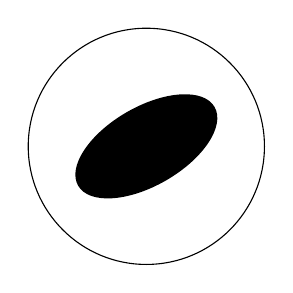
\begin{tikzpicture}
\draw (1,0) circle [radius=1.5];
\fill (1,0) circle [x radius=1cm, y radius=5mm, rotate=30];
\end{tikzpicture}

% 159
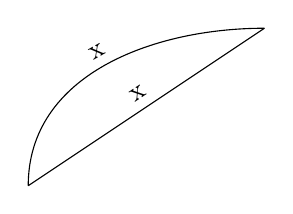
\begin{tikzpicture}
\draw (0,0) to [edge node={node [sloped,above] {x}}] (3,2);
\draw (0,0) to [out=90,in=180,
edge node={node [sloped,above] {x}}] (3,2);
\end{tikzpicture}

% 175
\tikz \shadedraw [shading=axis] (0,0) rectangle (1,1);
\tikz \shadedraw [shading=radial] (0,0) rectangle (1,1);
\tikz \shadedraw [shading=ball] (0,0) circle (.5cm);

% 234
\begin{tikzpicture}[level distance=8mm]
\node (root) {root}
child { node (a) {a} }
child { node (b) {b}
child { node (d) {d} }
child { node (e) {e} } }
child { node (c) {c} };
\begin{pgfonlayer}{background}
\node[fill=red!20,inner sep=0pt,ellipse,fit=(root) (b) (d) (e)] {};
\node[fill=blue!20,inner sep=0pt,ellipse,fit=(b) (c) (e)] {};
\end{pgfonlayer}
\end{tikzpicture}

% 238
\tikz [allow upside down]
\draw (0,0) .. controls +(up:2cm) and +(left:2cm) .. (1,3)
node foreach \p in {0,0.25,...,1} [sloped,above,pos=\p]{\p};

% 246
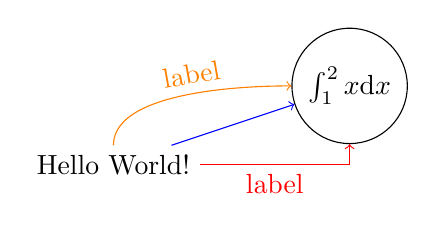
\begin{tikzpicture}
\path (0,0) node
 (x) {Hello World!}
(3,1) node[circle,draw](y) {\(\int_1^2 x \mathrm d x\)};
\draw[->,blue]
 (x) -- (y);
\draw[->,red]
 (x) -| node[near start,below] {label} (y);
\draw[->,orange] (x) .. controls +(up:1cm) and +(left:1cm) .. 
node[above,sloped] {label} (y);
\end{tikzpicture}

% % 249
% \begin{tikzpicture}[remember picture]
% \node (c) [circle,draw] {Big circle};
% \draw [overlay,->,very thick,red,opacity=.5]
% (c) to[bend left] (n1) (n1) -| (n2);
% \end{tikzpicture}

% % 346
% \tikzfading[name=fade inside,
% inner color=transparent!80,
% outer color=transparent!30]
% \begin{tikzpicture}
% % Checker board
% \fill [black!20] (0,0) rectangle (4,4);
% \path [pattern=checkerboard,pattern color=black!30] (0,0) rectangle (4,4);
% \shade [ball color=red] (3,3) circle (0.8);
% \shade [ball color=white,path fading=fade inside] (2,2) circle (1.8);
% \end{tikzpicture}

% 603
\begin{tikzpicture}
a big \draw [help lines] grid (3,2);
 \draw [red, dashed]
[postaction={decoration={text along path, text={a big juicy apple},
text align={align=right}}, decorate}]
 (0,0) .. controls (0,2) and (3,2) .. (3,0);
\end{tikzpicture}

% 754
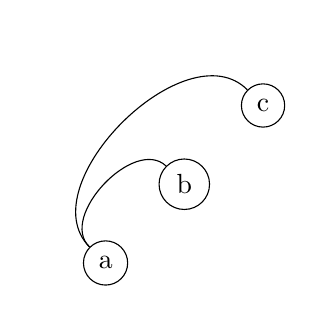
\begin{tikzpicture}[out=90,in=90,relative]
\node [circle,draw] (a) at (0,0) {a};
\node [circle,draw] (b) at (1,1) {b};
\node [circle,draw] (c) at (2,2) {c};
\path (a) edge (b)
edge (c);
\end{tikzpicture}

% % 841
% \tikz \datavisualization [
% school book axes,
% x axis={label=£x£},
% visualize as smooth line/.list={log, lin, squared, exp},
% every data set label/.append style={text colored},
% log= {pin in data={text’=£\log x£, when=y is -1}},
% lin= {pin in data={text=£x/2£, when=x is 2,
%       pin length=1ex}},
% squared={pin in data={text=£x^2£, when=x is 1.1,
%          pin angle=230}},
% exp= {label in data={text=£e^x£, when=x is -2}},
% style sheet=vary hue]
% data group {function classes};

% \end{comment}

%--------------------------------------------------------------------
% Vecchia versione
%--------------------------------------------------------------------

\begin{comment}

\chapter{Funzioni}

Riprendiamo ora il concetto di funzione, precedentemente studiato nel 
capitolo 
12 del secondo volume, approfondendone alcuni aspetti che ci saranno utili 
nel 
proseguo del nostro percorso.

\section{Definizione di funzione}
%label{}
\begin{definizione}
  Dati due insiemi \(A\) e \(B\) non vuoti definiti in \(\mathbb{R}\) è detta 
\(f\), \textsc{funzione reale di variabile reale}, una qualsiasi legge, 
applicazione o corrispondenza che associa a ogni elemento di \(A\) uno e un 
solo elemento di \(B\).
\end{definizione}

\begin{figure}[htpb!]
  \centering
  \includegraphics[width=0.55\textwidth]{img/1_funz.png}
  %%\caption{}
  %%\label{fig:1_1}
\end{figure}

Una funzione viene indicata:\\

\(f: A\to B  \)  tra insiemi   \(f: x\mapsto y\)   tra elementi  con \(x\in A 
\)  e \(y\in B\)\\

Dobbiamo pensare che \(x\) mediante la corrispondenza \(f\) diventa \(y\), 
l'elemento \(y\) è dunque l'\textsc{immagine} di \(x\) mediante la 
trasformazione 
\(f\); altrettanto e viceversa possiamo chiamare \(x\) \textsc{controimmagine} 
di 
\(y\).\\

L'elemento \(x\) viene dunque proiettato mediante una sua trasformazione che 
chiamiamo \(f\) nell'elemento \(y\) di \(B\), \(y\) risulta così dipendente da \(x\) 
perché determinata proprio in funzione di \(x\), variabile indipendente.\\

L'immagine \(y\) risulta propriamente in funzione di \(x\) e possiamo scrivere 
\(f(x)=y\) e la precedente espressione tra elementi diventa \(f: x\mapsto 
f(x)=y\).\\

Definiamo \(D\) \textsc{dominio} l'insieme \(A\) delle \(x\) e \(C\) 
\textsc{codominio} il sottoinsieme di \(B\) di tutte le immagini di \(x\), cioè 
di tutte e sole le \(y\) generate dalla trasformazione \(f\).\\

\begin{figure}[htpb!]
  \centering
  \includegraphics[width=0.55\textwidth]{img/2_funz.png}
  %\caption{}
  %\label{fig:1_2}
\end{figure}
%
Notiamo, nella figura precedente che mentre il dominio coincide con 
l'insieme 
di partenza il codominio è un sottoinsieme dell'insieme di arrivo.\\

%
%
%
\begin{esempio}
  Visualizziamo dominio e codominio della funzione \(f(x)=x^2\)
  \begin{figure}[htpb!]
  \centering
  \includegraphics[width=0.4\textwidth]{img/2a_funz.png}
  %\caption{}
  %\label{fig:1_2}
  \end{figure}
\end{esempio}

\begin{esempio}
  Visualizziamo dominio e codominio della funzione \(f(x)=\log{x}\)
  \begin{figure}[htpb!]
  \centering
  \includegraphics[width=0.4\textwidth]{img/2b_funz.png}
  %\caption{}
  %\label{fig:1_2}
  \end{figure}
\end{esempio}

\begin{esempio}
  Visualizziamo dominio e codominio della funzione \(f(x)=\frac{9}{x}\)
  \begin{figure}[htpb!]
  \centering
  \includegraphics[width=0.55\textwidth]{img/2c_funz.png}
  %\caption{}
  %\label{fig:1_2}
  \end{figure}
\end{esempio}

\newpage 
Per calcolare il dominio delle funzioni, vediamo una tabella riassuntiva 
dei 
possibili casi.\\

%%%%%%%%%%%%%%TABELLA DOMINIO FUNZIONI%%%%%%%%%%%%
\begin{table}

\raggedleft
%   \begin{tabularx}{1,2\textwidth}{XXX}
  \begin{tabularx}{\textwidth}{XXX}
  \toprule
  Funzione & Dominio  & Esempio \\
  \midrule
  
  \textbf{Funzioni razionali intere} 
\newline\(y=a_0x^n+a_1x^{n-1}+\dots+a_n\) 
  & \(\,\) \newline \(D=\mathbb{R}\) 
  & \(\,\) \newline \(y=x^3-x^2+2x+1\) \newline \(D=\mathbb{R}\) \\
  \midrule

  \textbf{Funzioni razionali fratte} \newline 
\(y=\frac{A(x)}{B(x)}\) \newline con \(A(x)\) e \(B(x)\) polinomi 
  & \(\mathbb{R}\) esclusi i valori che annullano \(B(x)\), cioè 
\newline \(B(x)\neq 0\)
  & \(\,\) \newline\(y=\frac{3+x^2}{x-5}\)\newline \(D= 
\mathbb{R}-\{5\}\) \\
  \midrule

  \textbf{Funzioni irrazionali} \newline \(y=\sqrt[n]{f(x)}\) 
\newline con \(n\in\mathbb{N},\,n>1\) 
  & \(\,\) \newline Se \(n\) è dispari il \(D\) è il \(D\) di \(f(x)\) 
\newline \newline Se \(n\) è pari, \newline\(D=\{x\in\mathbb{R}\vert 
f(x)\geq0\}\)
  & \(\,\) \newline \(y=\sqrt[3]{x^2-9}\)\newline \(D=\mathbb{R}\) 
\newline \newline \(y=\sqrt{x^2-1}\)\newline \(D=x^2\geq1=\)\newline 
\(=x\leq-1\lor x\geq1\) \\
  \midrule
  
  \textbf{Funzioni logaritmiche} \newline \(y=\log_af(x)\) 
\newline con \(a>0,\,a\neq1\) \newline \newline \(y=\log_{g(x)}(f(x))\) 
  & \(\,\) \newline \(D=\{x\in\mathbb{R}\vert f(x)>0\}\)\newline 
\newline \newline\(D=\{x\in\mathbb{R}\vert f(x)>0\land\)\newline\(\land 
g(x)>0\land g(x)\neq1\}\)
  & \(\,\) \newline \(y=\log(x+1)\)\newline \(D=x>-1\)\\
  \midrule
  
   \textbf{Funzioni esponenziali} \newline \(y=a^{f(x)}\) 
\newline con \(a>0,\,a\neq1\) \newline\newline  \(y={f(x)}^{g(x)}\) 
  & \(\,\) \newline \(D\) di \(f(x)\) \newline \newline \newline 
\(D=\{x\in\mathbb{R}\vert f(x)>0\}\land\) \(D\) di \(g(x)\)
  &  \(\,\) \newline\(y=3^{2x}\)\newline \(D= \mathbb{R}\) \newline  
\newline\(y=e^{\frac{1}{x+1}}\) \newline \(D=\mathbb{R}-\{-1\}\) \\
  \midrule
  
  \textbf{Funzioni potenza} \newline \(y=f(x)^a\) \newline con 
\(a\in\mathbb{R},\,a\neq0\) \newline \newline\(a\) intero positivo \newline 
\newline \(a\) intero negativo \newline  \newline \(a\) razionale \newline  
\newline\(a\) irrazionale positivo \newline \newline \(a\) irrazionale negativo 
  & \(\,\)  \newline  \newline  \newline  \newline  \(D\) di \(f(x)\) 
\newline  \newline \(D\) di \(f(x)\) con \(f(x)\neq0\)\newline \newline \(D\) di 
\(f(x)\) razionale \newline \newline \(D=\{x\in\mathbb{R}\vert 
f(x)\geq0\}\)\newline \newline \(D=\{x\in\mathbb{R}\vert f(x)>0\}\)
  & \(\,\)  \newline  \newline  \newline  \newline \(y=(x-1)^2\) 
\(D=\mathbb{R}\) \newline \newline \(y=(x-1)^{-2}\) \(D=x\neq1\) \newline 
\newline 
\(y=(x-1)^{1/2}=\sqrt{x-1}\) \(D=x\geq1\) \newline \(y=(x-1)^{\pi}\) \(D=x\geq1\) 
\newline \newline \(y=(x-1)^{-\pi}\) \(D=x>1\)\\
  \midrule

  \textbf{Funzioni goniometriche} \newline \(y=\sin{x}\), 
\(y=\cos{x}\) \newline \newline \(y=\tan x\), \(y=\sec x\) \newline  \newline 
\(y=\cot x\), \(y=\csc x\) 
  & \(\,\) \newline \(D=\mathbb{R}\) \newline  \newline 
\(D=\mathbb{R} -\bigl\{\frac{\pi}{2}+k\pi \bigr\}\)\newline \newline 
\(D=\mathbb{R} -\{k\pi\}\)
  &  \\
  \midrule
  
\end{tabularx}
\end{table}

\begin{table}   

\raggedleft   
\begin{tabularx}{\textwidth}{XXX}
  \midrule

  \textbf{Funzioni goniometriche inverse} \newline 
\(y=\arcsin{x}\), \(y=\arccos{x}\) \newline \newline \(y=\arctan x\), 
\(y=\text{arccot}\,x\)
  & \(\,\) \newline \newline \(D=[-1,1]\) \newline  \newline 
\(D=\mathbb{R}\)
  &  \\
  \midrule

  \textbf{Funzioni goniometriche composte} \newline 
\(y=\sin[f(x)]\), \(y=\cos [f(x)]\) \newline \newline \(y=\tan [f(x)]\) \newline 
\newline \newline \(y=\cot [f(x)]\) \newline  \newline \(y=\arcsin[f(x)]\), 
\newline \(y=\arccos [f(x)]\) \newline \newline \(y=\arctan [f(x)]\)
  & \(\,\) \newline \newline \(D\) di \(f(x)\) \newline  \newline 
\(D=\bigl\{x\in\mathbb{R}\vert f(x)\neq\frac{\pi}{2}+\newline+k\pi 
\bigr\}\)\newline \newline \(D=\{x\in\mathbb{R}\vert f(x)\neq k\pi\}\) 
\newline 
\newline \(D=\{x\in\mathbb{R}\vert -1\leq f(x)\leq\newline\leq1\}\) \newline 
\newline \(D\) di \(f(x)\)
  & \(\,\) \newline \newline \newline \(y=\tan[2x-1]\) \newline 
\(2x-1\neq \frac{\pi}{2}+k\pi\) \newline\(D=x\neq\frac{\pi+1+k\pi}{2}\)  
\newline 
\newline \newline  \(y=\arcsin[x-1]\) \newline \(-1\leq x-1\leq1\)\newline 
\(0\leq 
x\leq2\)\newline \newline\(y=\arctan [\frac{x+2}{x+3}]\) \newline 
\(D=\mathbb{R}-\{-3\}\)
 \\

  \bottomrule
\end{tabularx}
\end{table}
\newpage

\section{La rappresentazione di una funzione}
%label{}
Una funzione può essere rappresentata in diversi modi, i principali sono:
\begin{itemize}
  \item \textsc{Rappresentazione tabulare}\\
Le funzioni empiriche vengono ricostruite con una tabella in cui ad ogni 
\(y\) 
corrisponde un certo \(x\). Ad esempio pensiamo ad una tabella che dà la 
temperatura ora per ora in un certo luogo.
%
  \item \textsc{Rappresentazione analitica}\\
La funzione è espressa mediante un insieme di operazioni matematiche che 
applicate in un certo ordine ad \(x\) restituiscono un corrispondente valore 
di 
\(y\). Esempi ne sono \(y=\log{(x+2)}\), \(y=2x^3+3\) o \(y=\sin{x}+2^x\), cioè le 
espressioni, scritte in linguaggio matematico, che siamo abituati a 
trattare.
%
  \item \textsc{Rappresentazione grafica}\\
La funzione è rappresentata come una corrispondenza \(x-\)y su un grafico 
cartesiano; in particolare, ricordiamo che: il grafico di una funzione \(f 
:A\to B\) è l'insieme di tutte le coppie ordinate \((x;y)\) che si ottengono 
prendendo un valore \(x\) in \(A\) e trovando il corrispondente valore \(y=f(x)\) 
in \(B\). Ogni coppia ordinata rappresenta un punto nel piano cartesiano 
\(\mathbb{R}^2\).
\end{itemize}

\section{Le proprietà di una funzione}
%label{}
Una funzione, a seconda, del modo in cui gli elementi del dominio 
corrispondono agli elementi del codominio si può definire 
\textsc{iniettiva}, 
\textsc{suriettiva} e \textsc{biiettiva} (o \textsc{biunivoca}).\\

\begin{definizione}
Una funzione da \(A\) a \(B\) si dice \textsc{iniettiva} se ogni elemento di 
\(B\) 
è immagine di \underline{al più} un elemento di \(A\);\\


\(f : A\to B\) è iniettiva se  \(\forall x_1,\,x_2\in A ,\,x_1\neq 
x_2\Rightarrow f(x_1 )\neq f(x_2)\)
\end{definizione}

\begin{figure}[htpb!]
  \centering
  \includegraphics[width=0.55\textwidth]{img/3_funz.png}
  %\caption{}
  %\label{fig:1_2}
\end{figure}

\begin{definizione}
Una funzione da \(A\) a \(B\) si dice \textsc{suriettiva} quando ogni elemento 
di 
\(B\) è immagine di \underline{almeno un} elemento di \(A\);\\

\(f: A\to B\) è suriettiva se \(\forall y\in B, \exists x\in A \mid f(x)=y\)
\end{definizione}

\begin{figure}[htpb!]
  \centering
  \includegraphics[width=0.55\textwidth]{img/4_funz.png}
  %\caption{}
  %\label{fig:1_2}
\end{figure}

Il fatto che una funzione sia o non sia suriettiva dipende da come si 
sceglie 
l'insieme di arrivo. Se lo si sceglie coincidente con il codominio la 
funzione è suriettiva.\\
%
\begin{definizione}
Una funzione da \(A\) a \(B\) è \textsc{biiettiva} (o \textsc{biunivoca}) 
quando 
è sia iniettiva sia suriettiva.\\
\end{definizione}

\begin{figure}[htpb!]
  \centering
  \includegraphics[width=0.55\textwidth]{img/5_funz.png}
  %\caption{}
  %\label{fig:1_2}
\end{figure}

\begin{esempio} Quando una funzione è biettiva?\\
Una funzione biiettiva è ad esempio una qualsiasi retta. Una retta è 
infatti 
sia iniettiva, che biettiva di dominio \(\mathbb{R}\) e codominio 
\(\mathbb{R}\).\\
\end{esempio}

Una funzione biiettiva viene anche detta biiezione o corrispondenza 
biunivoca 
fra gli insieme \(A\) e \(B\). Tale relazione tra insiemi è molto forte e 
specifica in quanto ad ogni elemento di \(A\) viene associato un solo 
elemento 
di \(B\) e, reciprocamente, ad ogni elemento di \(B\) è associato un solo 
elemento di \(A\), in una relazione uno a uno. Per tale ragione, la relazione 
tra i due insiemi viene indicata con una doppia freccia \(A\leftrightarrow 
B\).
%
\section{Le caratteristiche di una funzione}
%label{}
Analizziamo ora le caratteristiche che può manifestare una funzione, 
qualità 
che può presentare il suo andamento e che possono contraddistinguerne la 
forma del grafico.

\subsection{Monotonia}
%label{}
La caratteristica della monotonia vuole evidenziare l'andamento 
\textsc{crescente} o \textsc{decrescente} di una funzione; la monotonia 
studia il comportamento della variabile dipendente \(y\) all'aumentare della 
variabile indipendente \(x\). All'aumentare dell'ascissa se aumenta anche 
l'ordinata diremo che la funzione cresce, se l'ordinata diminuisce diremo 
che 
la funzione decresce. Vediamo e puntualizziamo meglio.\\

\begin{definizione}
Una funzione \(y=f(x)\) di dominio \(D\), si dice \textsc{crescente in senso 
stretto} in un intervallo \(I\), sottoinsieme di \(D\), se\\

\(\forall x_1,x_2\in I\)  con \(x_1<x_2 \) si ha \(f(x_1)<f(x_2)\)\\
\end{definizione}

\begin{figure}[htpb!]
  \centering
  \includegraphics[width=0.55\textwidth]{img/funz_6.png}
  %\caption{}
  %\label{fig:1_2}
\end{figure}
%
\begin{definizione}
Una funzione è non decrescente o \textsc{crescente} in senso lato in un 
intervallo \(I\), sottoinsieme di \(D\), se\\

\(\forall x_1,x_2\in I\)  con \(x_1<x_2 \) si ha \(f(x_1)\leq f(x_2)\)\\
%
\end{definizione}
%
%
%

\begin{definizione}
Una funzione \(y=f(x)\) di dominio \(D\), si dice \textsc{decrescente in senso 
stretto}, in un intervallo \(I\), sottoinsieme di \(D\), se\\

\(\forall x_1,x_2\in I\)  con \(x_1<x_2 \) si ha \(f(x_1)> f(x_2)\)\\

\end{definizione}

\begin{figure}[htpb!]
  \centering
  \includegraphics[width=0.55\textwidth]{img/funz_7.png}
  %\caption{}
  %\label{fig:1_2}
\end{figure}
%

\begin{definizione}
Una funzione è non crescente o \textsc{decrescente} in senso lato in un 
intervallo \(I\), sottoinsieme di \(D\), se\\

\(\forall x_1,x_2\in I\)  con \(x_1<x_2 \) si ha \(f(x_1)\geq f(x_2)\)\\
\end{definizione}

Una funzione, quindi, si dice monotòna in un intervallo \(I\) del suo dominio 
se in \(I\) è sempre crescente o decrescente.\\

\begin{esempio}
Individuiamo gli intervalli in cui la funzione rappresentata risulta 
crescente o decrescente.\\
Negli intervalli finiti \(x_1<x<x_2\), \(x_3<x<x_4\) la funzione risulta essere 
crescente; negli intervalli finiti \(x_2<x<x_3\), \(x_4<x<x_5\).
% 
\begin{figure}[htpb!]
  \centering
  \includegraphics[width=0.4\textwidth]{img/funz_8.png}
  %\caption{}
  %\label{fig:1_2}
\end{figure}
\end{esempio}
\subsection{Parità}
%label{}
La caratteristica della parità va a verificare se il grafico della funzione 
che stiamo studiando è simmetrico rispetto all'asse delle \(Y\), cioè il 
grafico è speculare rispetto all'asse, o se il grafico della funzione è 
simmetrico rispetto all'origine. Nel primo caso parleremo di 
\textsc{parità} 
della funzione, nel secondo caso parleremo di \textsc{disparità} della 
funzione.\\

Ovviamente non tutte le funzioni presenteranno questa simmetria, possiamo 
però individuare delle condizioni che, se presenti nella funzione, ci 
assicurano che questa è pari o dispari.\\

\begin{definizione}
Sia data una funzione \(y=f(x)\), avente dominio \(D\) tale che per ogni \(x\in 
D\) 
anche \(-x\in D\). Una funzione si dice \textsc{pari} in \(D\) se \\
\[f(-x)=f(x)\]
per ogni \(x\in D\).
\end{definizione}

\begin{figure}[htpb!]
  \centering
  \includegraphics[width=0.5\textwidth]{img/funz_9.png}
  %\caption{}
  %\label{fig:1_2}
\end{figure}
%

Se una funzione è pari, il suo grafico è simmetrico rispetto all'asse \(Y\). 
Infatti se \(P(x;y)\) appartiene al grafico anche \(P'(-x;y)\) vi appartiene. 
Sottolineiamo ancora che la condizione di parità per una funzione è \(f(-x)= 
f(x)\).\\   

\begin{esempio} Verificare se una funzione è o non è pari.\\
Per verificare se una funzione è pari basta sostituire nella funzione \(-x\) 
al 
posto di \(x\) e verificare se la nuova \(f(-x)\) è uguale alla funzione di 
partenza, cioè se \(f(-x)=f(x)\). Se prendiamo la funzione 
\[f(x)=\frac{x^2+3}{x+2}\] \underline{non} è pari, infatti 
\[f(-x)=\frac{(-x)^2+3}{(-x)+2}=\frac{x^2+3}{-x+2}\neq f(x).\]
\end{esempio}

\begin{definizione}
Sia data una funzione \(y=f(x)\), avente dominio \(D\) tale che per ogni \(x\in 
D\) 
anche\( -x\in D.\) Una funzione si dice \textsc{dispari} in \(D\) se\\
\[f(-x)=-f(x)\]
per ogni \(x\in D\).
\end{definizione}

\begin{figure}[htpb!]
  \centering
  \includegraphics[width=0.5\textwidth]{img/funz_10.png}
  %\caption{}
  %\label{fig:1_2}
\end{figure}
%

Se una funzione è dispari, il suo grafico è simmetrico rispetto 
all'origine. 
Infatti se \(P(x;y)\) appartiene al grafico anche \(P'(-x;-y)\) vi appartiene. 
Sottolineiamo ancora che la condizione di disparità per una funzione è 
\(f(-x)= -f(x)\). \\

\begin{esempio} Verificare se una funzione è o non è dispari.\\
Per verificare se una funzione è dispari basta sostituire nella funzione 
\(-x\) 
al posto di \(x\) e verificare se la nuova \(f(-x)\) è uguale alla funzione di 
partenza cambiata di segno, cioè se \(f(-x)=-f(x)\). Se prendiamo la funzione 
\[f(x)=\frac{x}{x^2+2}\] è dispari, infatti 
\[f(-x)=\frac{(-x)}{(-x)^2+2}=\frac{-x}{x^2+2}=-\frac{x}{x^2+2}= -f(x).\]
\end{esempio}

\subsection{Periodicità}
%label{}
La periodicità di una funzione specifica se questa si ripete uguale a sé 
stessa ad intervalli regolari.\\

\begin{definizione}
Una funzione \(y=f(x)\), \(f(x): A\to \mathbb{R}\) si dice \textsc{periodica} 
di 
periodo \(T>0\) di periodo \(T>0\) se\(\forall x\in A\rightarrow (x+T)\in A\)e 
possiamo scrivere 
 \[f(x+T)=f(x)\]\\
\end{definizione}

\begin{figure}[htpb!]
  \centering
  \includegraphics[width=0.45\textwidth]{img/funz_11a.png} \quad 
  \includegraphics[width=0.45\textwidth]{img/funz_11b.png}
  %\caption{}
  %\label{fig:1_2}
\end{figure}


\begin{esempio} Calcolare il periodo di una funzione.\\
Calcoliamo il periodo della  funzione goniometrica \[y=\sin{7x}\] con due 
possibili procedure:
\begin{itemize}
  \item[\textsf{Procedura a)}] La funzione ha per definizione periodo 
\(T\) se, con \(k\) intero,
\[\sin[(7(x+kT)]=\sin4x\]
cioè,
\[\sin[(7x+7kT)]=\sin4x\]
poichè la funzione seno ha periodo \(2\pi\), allora
\[\sin[7x+7kT]=\sin[7x+2k\pi]\]
e l'uguaglianza è quindi valida se \(7T=2\pi\) da cui
\[T=\frac{2\pi}{7}.\]

  \item[\textsf{Procedura b)}] La funzione \(y'=\sin7x'\) viene dalla 
trasformazione della funzione \(y=\sin x\), che ha periodo \(T=2\pi\), mediante 
una sostituzione \(7x'=x\), ovvero \(x'=\frac{x}{7}\). Se l'asse delle ascisse 
viene così contratto di un fattore \(\frac{x}{7}\), il periodo \(T'\) subirà la 
stessa contrazione e pertanto è pari a 
\[T'=\frac{x}{7}(2\pi)=\frac{2\pi}{7}\]
\end{itemize}
\end{esempio}

Se due funzioni \(f(x)\) e \(g(x)\) hanno periodi diversi \(T_f\) e \(T_g\), 
rispettivamente, le funzioni \(f(x)\pm g(x)\), \(f(x)\cdot g(x)\) e 
\(\frac{f(x)}{g(x)}\) hanno un periodo pari al m.c.m. tra \(T_f\) e \(T_g\) 
nell'ipotesi che \(\frac{T_f}{T_g}\) sia un numero razionale e diverso da 1. 
Se il rapporto è irrazionale le precedenti combinazioni di funzioni non 
sono periodiche. Se \(T_f=T_g\) il periodo globale è minore o uguale del 
periodo comune.\\

\begin{esempio} Calcolare il periodo di combinazioni di funzioni periodiche e 
non periodiche.\\
  \begin{itemize}
  \item[a)] \(f(x)=\sin x+\cos 3x\) è periodica di \(2\pi\) che è 
il m.c.m. tra \(T_f=2\pi\) e \(T_g=\frac{2}{3}\pi\).
  
  \item[b)] \(f(x)=\sin x+\cos \pi x\) non è periodica perché il 
rapporto \(\frac{T_f}{T_g}\notin \mathbb{Q}\), infatti \(T_f=2\pi\) e \(T_g=2\), 
per cui \(\frac{2\pi}{2}=\pi\notin\mathbb{Q}\)
  
  \item[c)] \(f(x)=\sin \frac{x}{2}-\cos 3x+\tan x\) dove 
\(T_{\sin \frac{x}{2}}=4\pi\), \(T_{\cos 3x}=\frac{2}{3}\pi\), \(T_{\tan}=\pi\)
  
  \item[d)] Se consideriamo la funzione 
\[f(x)=\frac{1}{\log[\sin x]}\] il periodo è \(2\pi\)
\end{itemize}
\end{esempio}

Se una funzione è periodica i valori delle sue ordinate si ripetono con 
regolarità, quindi per studiarne l'andamento su tutto l'asse reale, basterà 
studiarne l'andamento in un singolo periodo. Ripetiamo ancora che la 
condizione di parità per una funzione è \(f(x+T)=f(x)\) con \(T\) periodo.
%
%
\subsection{Limitatezza}
%label{}
La limitatezza di una funzione valuta se le ordinate di una funzione 
raggiungono un valore massimo e un valore minimo, oppure non hanno un 
limite.\\


\begin{definizione}
Consideriamo una funzione \(f: A\to \mathbb{R}\), la funzione si dice:
  \begin{itemize}
  \item[\(\rhd\)]\textsc{limitata superiormente} se il suo 
codominio \(f(A)\) ha un limite superiore \(k\):
\[\exists k\in \mathbb{R} \vert \forall x\in A,\, k\geq f(x)\] 
  \item[\(\rhd\)]\textsc{limitata inferiormente} se il suo 
codominio f(A) ha un limite inferiore \(k\): 
\[\exists k\in \mathbb{R} \vert \forall x\in A,\, k\leq f(x)\]

  \item[\(\rhd\)]\textsc{limitata} se il suo codominio \(f(A)\) è 
limitato sia superiormente che inferiormente:
\[\exists k\in \mathbb{R},k>0\vert\forall x\in A, \vert f(x)\vert \leq k\]
\end{itemize}

Se una funzione non è limitata da un valore del codominio \(k\) si dirà 
illimitata, in particolare:
  \begin{itemize} 
  \item[\(\rhd\)] \textsc{Illimitata superiormente} se il suo 
codominio \(f(A)\) \underline{non} è limitato superiormente;
  \item[\(\rhd\)] \textsc{Illimitata inferiormente} se il suo 
codominio \(f(A)\) \underline{non} è limitato inferiormente;
  \item[\(\rhd\)] \textsc{Illimitata} se il suo codominio \(f(A)\) 
\underline{non} è limitato superiormente \underline{né} inferiormente.
  \end{itemize}
\end{definizione}
%
\begin{esempio} Determinare la limitatezza o illimitatezza di funzioni.\\
In (a) La funzione \(f(x)=\log(x)\) è illimitata: né superioremente né 
inferiormente limitata; in (b) La funzione è limitata inferiormente e 
illimitata superiormente; in (c) La funzione \(f(x)=\sin{x}\) è limitata sia 
superiormente che inferiormente; in (d) La funzione \(f(x)=x^2\) è limitata 
inferiormente e illimitata superiormente.
\begin{figure}[h]
  \centering
  \includegraphics[width=0.85\textwidth]{img/funz_12a.png}
  %\label{fig:1_2}
\end{figure}
\end{esempio}
\newpage
\section{La classificazione delle funzioni}
%label{}
Classifichiamo le possibili funzioni che incontreremo o abbiamo incontrato in 
base alle operazioni che compaiono nella loro espressione analitica. Se 
nell'espressione analitica di una funzione compaiono le operazioni di 
addizione, sottrazione, moltiplicazione, divisione, elevamento a potenza con 
esponente razionale o estrazione di radice siamo di fronte ad una 
\textsc{funzione algebrica}.\\

Le funzioni che non possono essere rappresentate usando solamente le 
operazioni precedentemente ricordate si dicono \textsc{trascendenti}. Tra le 
più note funzioni trascendenti ricordiamo le funzioni goniometriche, quelle 
esponenziali e quelle logaritmiche.\\

A seconda che le funzioni algebriche contengano o meno l'operazione di radice 
e l'operazione di divisione suddividiamo le funzioni algebriche in 
\textsc{razionali fratte}, \textsc{razionali intere} o polinomiali, 
\textsc{irrazionali fratte} e \textsc{irrazionali intere}. \\

\textsf{MEMO!!} Per non creare equivoci ricordiamo che una funzione è 
definita fratta quando il denominatore contiene la variabile indipendente 
\(x\), è invece definita irrazionale quando tale variabile appare sotto il 
segno di radice.\\

% TODO non compila!!!!!!!!!!!!!!!!!!!!!!!!!!!!!!!!!!!!!!!!!!!!!!!!!!!
% \Tree [.FUNZIONI [.\textbf{algebriche}  [.razionali fratte intere 
% !{\qbalance} ] [.irrazionali fratte intere !{\qbalance} ] ] 
% [.\textbf{trascendenti} goniometriche esponenziali logaritmiche ] ] \\


\begin{esempio} Classificazione di funzioni.\\
Classifichiamo le seguenti funzioni: 
  \begin{itemize}
  \item[a)] \(f(x)=\frac{\sqrt{(x+5)}}{3}\) è una funzione 
irrazionale intera, infatti pur avendo un denominatore, questo non contiene 
la variabile indipendente \(x\);
  
  \item[b)] \(g(x)=e^{\frac{x}{x-1}}\) è una funzione 
trascendente di tipo esponenziale;

  \item[c)] \(h(x)=\sqrt{2}x+4x\) è una funzione razionale 
intera, in quanto la radice compare solo nel numero irrazionale  a 
coefficiente della \(\sqrt{2}\) \(x\).
  \end{itemize}
\end{esempio}

\section{Funzioni inverse, composte e uguali}
%label{}
Nella rappresentazione insiemistica studiata finora abbiamo sempre visto le 
frecce partire dall'insieme \(A\) per arrivare nell'insieme \(B\). Esiste una 
possibile lettura al contrario? Se le frecce partissero da \(B\), dalle \(y\) per 
arrivare alle \(x\), ci troveremmo ancora in presenza di una funzione?

\begin{definizione}
Sia \(f : A\to B\) una funzione biiettiva. Si dice funzione inversa di \(f\) la 
funzione \(f^{-1} : B\to A\) che associa a ogni \(y\) di \(B\) il valore \(x\) di \(A\) 
tale che \(y=f(x)\).
\end{definizione}

\begin{figure}[htpb!]
  \centering
  \includegraphics[width=0.45\textwidth]{img/funz_12.png} 
  %\caption{}
  %\label{fig:1_2}
\end{figure}

Notiamo che se una funzione ammette inversa si dice \textsc{invertibile}. 
Significativa è, poi, la relazione tra i codomini e i domini delle due 
funzioni, \(f\) e la sua inversa: il dominio di \(f^{-1}\) è l'immagine di \(f\) e 
l'immagine di \(f^{-1}\) è il dominio di \(f\).\\

\begin{esempio} Calcolare  e graficare l'inversa di una funzione, verificando 
che sia invertibile.\\ 
Consideriamo la funzione biiettiva \(f:\mathbb{R}\to\mathbb{R}\) definita da
\[f(x)=y=3x+2\]
Possiamo ottenere la sua inversa \(f^{-1}\) nel seguente modo:
  \begin{itemize}
  \item ricaviamo \(x\) in funzione di \(y\) dalla relazione 
precedente
\[x=\frac{y-2}{3}\]
  \item sostituiamo la \(x\) con \(y\) e viceversa.
  \begin{figure}[htpb!]
  \centering
  
\includegraphics[width=0.5\textwidth]{img/funz_13.png} 
  %\caption{}
  %\label{fig:1_2}
  \end{figure}
  \item notiamo che il grafico della funzione inversa
\[f^{-1}(x)=\frac{x-2}{3}\]
è simmetrico a quello di \(f(x)\) rispetto alla bisettrice del primo e terzo 
quadrante, la retta di equazione \(y=x\)
  \end{itemize}
\end{esempio}

\begin{esempio} Disegnare l'inversa di una funzione che originariamente non 
sia invertibile nel suo dominio. 

La funzione \(f:\mathbb{R}\to\mathbb{R}\) tale che \[f(x)=x^2+1\].
\begin{itemize}
  \item \(f\) non ammette funzione inversa perché non è biiettiva, in 
quanto non è iniettiva.
  \begin{figure}[htpb!]
  \centering
  
\includegraphics[width=0.45\textwidth]{img/funz_14a.png} %\quad
  
%\includegraphics[width=0.7\textwidth]{img/funz_14b.png} \quad
  
%\includegraphics[width=0.7\textwidth]{img/funz_14c.png} 
  %\caption{}
  %\label{fig:funz_14abc}
  \end{figure}
  \item Se \(f\) non è biiettiva e quindi non è invertibile, possiamo 
operare una \textsc{restrizione del dominio} a un sottoinsieme in cui \(f\) 
risulti biiettiva.
  \begin{figure}[htpb!]
  \centering
  
%\includegraphics[width=0.7\textwidth]{img/funz_14a.png} %\quad
  
\includegraphics[width=0.45\textwidth]{img/funz_14b.png} %\quad
  
%\includegraphics[width=0.7\textwidth]{img/funz_14c.png} 
  %\caption{}
  %\label{fig:funz_14abc}
  \end{figure}
  \item Scelgo solo una parte del dominio che chiamo \(A\) e disegno 
l'inversa riflettendo la porzione di funzione biiettiva rispetto alla 
bisettrice del primo e terzo quadrante, la retta di equazione \(y=x\).
  \begin{figure}[htpb!]
  \centering
  
%\includegraphics[width=0.7\textwidth]{img/funz_14a.png} \quad
  
%\includegraphics[width=0.7\textwidth]{img/funz_14b.png} %\quad
  
\includegraphics[width=0.45\textwidth]{img/funz_14c.png} 
  %\caption{}
  %\label{fig:funz_14abc}
  \end{figure}
\end{itemize}
\end{esempio}

Come visto negli esempi precedenti, il grafico della funzione \(f^{-1}\), 
inversa della funzione \(f\), è il simmetrico di \(f\) rispetto alla bisettrice 
del primo e terzo quadrante.\\

Anche se sappiamo che l'inversa di una certa funzione deve essere simmetrica 
rispetto ad essa, trovare l'inversa di una determinata funzione e in 
particolar modo la sua forma analitica può non essere immediato. Forniamo 
quindi una procedura.\\

%\begin{procedura}
\textbf{Procedura 1.1} Determinare l'inversa di una funzione data:% 
\textcolor{blue}{[vedi la procedura a pag 100 vol3]}
\begin{enumerate}
  \item Si verifica che \(f(x)\) è invertibile;
  \item Si esplicita la \(f\) rispetto a \(x\);
  \item Nella forma appena trovata si sostituisce \(x\) con \(y\) e \(y\) con 
\(x\).
\end{enumerate}
%end{procedura}
  
\begin{esempio}
Invertiamo la funzione: \(f(x)=y=\sqrt[3]{x}-1\)
\begin{enumerate}
  \item La funzione è invertibile perché è strettamente crescente in 
tutto il dominio \(\mathbb{R}\).
  \item Esplicitiamo la funzione rispetto a \(x\):\\
   \(y=\sqrt[3]{x}-1\rightarrow y+1=\sqrt[3]{x}\rightarrow(y+1)^3=x\)
  \item Infine otteniamo: \(f^{-1}(x)=y=(x+1)^3\)
\end{enumerate}
\end{esempio}

\begin{esempio}
Invertiamo la funzione: \(f(x)=y=e^{x+1}-1\)
\begin{enumerate}
  \item La funzione è invertibile perché è strettamente crescente in 
\(\mathbb{R}\).
  \item Esplicitiamo la funzione rispetto a \(x\):\\
   \(y=e^{x+1}-1\rightarrow y+1=e^{x+1}\rightarrow 
\ln(x+1)=\ln(e^{x+1})\rightarrow \ln(y+1)-1=x\).\item Infine otteniamo: 
\(f^{-1}(x)=y=\ln(x+1)-1\).
\end{enumerate}
\end{esempio}

Studiate le funzioni inverse discutiamo ora un'operazione tra funzioni che ci 
consentirà di creare funzioni complesse a partire da funzioni semplici: 
questa operazione si chiama \textsc{composizione di funzioni} e il suo 
risultato sarà una nuova funzione detta composta.\\

%
\begin{definizione} 
Date le funzioni \(f : A\to B\) e \(g : B\to C\) si dice funzione composta 
\(f\circ g\) la funzione:   \((g\circ f)(x)=g(f(x))\) che associa ad ogni 
elemento di \(A\) un elemento di \(C\) in modo che
  \begin{itemize}
  \item all'elemento \(x\in A\) corrisponde mediante \(f\), 
l'elemento \(f(x)\in B\)
  \item all'elemento \(f(x)\in B\) corrisponde, mediante \(g\), 
l'elemento \(g(f(x))\in C\)
  \end{itemize}
affinché sia possibile calcolare \(g(f(x))\), \(f(x)\) deve appartenere al 
dominio di \(g\). Il dominio di \(g\circ f\) è costituito da tutti gli elementi 
del dominio di \(f\) tali che \(f(x)\) appartiene al dominio di \(g\).
\end{definizione}

\begin{figure}[htpb!]
  \centering
  \includegraphics[width=0.55\textwidth]{img/funz_15.png} 
  %\caption{}
  %\label{fig:funz_14abc}
\end{figure}
%

La simbologia \(g\circ f\) si legge <<\(g\) composto \(f\)>> o <<\(g\) dopo \(f\)>>; 
\(g(f(x))\) si legge <<\(g\) di \(f\) di \(x\)>>.\\
 
Per quanto riguarda le proprietà di questa operazione tra funzioni notiamo 
che la composizione è associativa: \((f\circ g)\circ h=f\circ (g\circ h)\), ma 
in generale non commutativa \(g\circ f\neq f\circ g.\) \\

\begin{esempio} 
Date le due funzioni \(f(x)=\sqrt{x}\) e \(g(x)= x+5\), determiniamo le funzioni 
composte \(g\circ f\) e \(f\circ g\).
Abbiamo \(g\circ f=g(f(x))=g(\sqrt{x})=\sqrt{x}+5\) e il dominio  della 
funzione ottenuta è \(x\geq0\). Otteniamo l'altra composta con un procedimento 
analogo \(f\circ g=f(g(x))=f(x+5)=\sqrt{x+5}\) e il suo dominio è \(x\geq5\). La 
diversità delle due funzioni ottenute ci conferma la non commutatività 
dell'operazione di composizione.\\
\end{esempio}

\textbf{Posso comporre una funzione con la sua inversa?}\\
Sia \(f\) una funzione invertibile di dominio \(D\) e immagine \(I\), con \(f^{-1} \) 
la sua inversa.
Consideriamo la composta \(f^{-1}\circ f\), cioè \(f^{-1}\) dopo \(f\): \(x\) va in 
\(f(x)\) che a sua volta va in \(x\), \(f^{-1}(f(x))=x\), \(\forall x\in D\) 
\(f^{-1}\circ f\) è la funzione identità in \(D\), analogamente anche 
\(f(f^{-1}(x))=x\), \(f\circ f^{-1}\) è l'identità in \(I\). Ricordiamo che la 
funzione identità è una particolare funzione che associa ad ogni \(x\) la \(x\) 
stessa, cioè associa ad ogni elemento del dominio, lo stesso elemento nel 
codominio.\\

\begin{definizione}
Due funzioni \(f\) e \(g\) si dicono uguali se hanno lo stesso dominio \(D\) e 
risulta \[f(x)=g(x)\] \(\forall x\in D\).\\
\end{definizione}
 
\begin{esempio}
Vediamo un esempio di funzioni uguali e non uguali. Le due funzioni
\[f(x)=\frac{\sqrt{x}}{\sqrt{x^2+4}}\] e \[g(x)=\sqrt{\frac{x}{x^2+4}}\]
sono uguali perchè hanno lo stesso dominio (\(x\geq0\)) e risulta:
\[\frac{\sqrt{x}}{\sqrt{x^2+4}}=\sqrt{\frac{x}{x^2+4}}\] per ogni \(x\geq0\).
Vediamo un contoesempio di funzioni uguali. Le due funzioni
\[f(x)=\frac{\sqrt{x}}{\sqrt{x+4}}\] e \[g(x)=\sqrt{\frac{x}{x+4}}\]
non sono uguali perché hanno dominio diverso: la funzione \(f\) è definita per 
\(x\geq0\), mentre la funzione \(g\) è definita per \(x<-4\lor x\geq 0\).
\[\frac{\sqrt{x}}{\sqrt{x^2+4}}=\sqrt{\frac{x}{x^2+4}}\] per ogni \(x\geq0\).
\end{esempio}


\end{comment}








